\documentclass[a4paper]{amsart}
\usepackage{amsmath,amsxtra,amsthm,amssymb,graphics,mathrsfs}
\usepackage{mathtools}
\usepackage[margin=2.7cm]{geometry}
\usepackage{enumerate}
%\usepackage{authblk} %For email address in title
\usepackage{stmaryrd}
%\usepackage{pdflscape} %landscape pages
\usepackage{indentfirst}
\usepackage{capt-of}
\usepackage{dsfont}
%\usepackage{enumitem}
\usepackage{setspace}
\usepackage{caption}
\usepackage[font+=large]{subcaption}
\usepackage[all]{xy}
\usepackage{bbm}
%\usepackage{slashbox}
\usepackage{graphicx}
\usepackage{xcolor}
\usepackage{verbatim} %Allow comments
\usepackage[notref,notcite]{showkeys}
\usepackage[bookmarks=true, colorlinks=true,linkcolor=black, anchorcolor=black,citecolor=black, urlcolor=black, 
bookmarksopenlevel=3]{hyperref}
%\usepackage{ytableau}
%\usepackage{genyoungtabtikz}
\usepackage{tikz}
\usetikzlibrary{patterns}
\usetikzlibrary{calc}
\usetikzlibrary{decorations.text}
\usetikzlibrary{decorations.shapes}
\usetikzlibrary{decorations.markings}
\usetikzlibrary{decorations.pathreplacing}

\numberwithin{equation}{subsection}

\newcount\tableauRow\newcount\tableauCol
\newcommand\drawtbx[2]{%
	\begin{scope}[shift={#2}]
    \tableauRow=0
    \foreach \Row in {#1} {
       \tableauCol=1
       \foreach\k in \Row {
          \draw(\the\tableauCol,\the\tableauRow)+(-.5,-.5)rectangle++(.5,.5);
          \draw(\the\tableauCol,\the\tableauRow)node{\k};
          \global\advance\tableauCol by 1
       }
       \global\advance\tableauRow by -1
    }
	\end{scope}
}

%\setlength{\parindent}{4mm}
%\setlength{\parskip}{12pt}

%\newtheoremstyle{all}{12pt}{0pt}{}{}
%{\bfseries}{}{\newline}{\thmname{#1}\thmnumber{ #2}\thmnote{ (#3)}}
%\theoremstyle{all}

%%%DEFINE USUAL THEOREM ENVIRONMENTS
\newtheorem{theorem}{Theorem}[section]
\newtheorem{proposition}[theorem]{Proposition}
\newtheorem{lemma}[theorem]{Lemma}
\newtheorem{corollary}[theorem]{Corollary}
\newtheorem*{proposition*}{Proposition}
\newtheorem*{theorem*}{Theorem}
\newtheorem*{conjecture*}{Conjecture}

\theoremstyle{definition}
\newtheorem{remark}{Remark}
\newtheorem{definition}[theorem]{Definition}
\newtheorem{notation}[theorem]{Notation}
\newtheorem{example}[theorem]{Example}
\newtheorem{def-prop}[theorem]{Definition-Proposition}
%\linespread{1.5}

%%%USE \label{1} TO FLAG LOCATIONS AND \ref{1} TO RETRIEVE
%%%ASTERISK * TO STOP NUMBERING
%%%{enumerate}{itemize}{tabular}{pmatrix}{align}{equation}
%%%USE \cite[pg]{Ref. in doc.} TO CITE REF IN PAPER.

%%%MATH OPERATORS
\DeclareMathAlphabet{\mathpzc}{OT1}{pzc}{m}{it}
%%%\DeclareMathOperator{Your Symbol}{How is it}
\DeclareMathOperator{\tensor}{\otimes}
\DeclareMathOperator{\isom}{\cong}
\DeclareMathOperator{\I}{\mathcal{I}}
\DeclareMathOperator{\F}{\mathbb{F}}
\DeclareMathOperator{\eS}{\mathscr{S}}
\DeclareMathOperator{\Tee}{\mathscr{T}}
\DeclareMathOperator{\T}{\mathbbmss{T}}
\DeclareMathOperator{\Z}{\mathbb{Z}}
\DeclareMathOperator{\B}{\mathbbm{B}}
\DeclareMathOperator{\sB}{\mathbbm{b}}
%Category
%\DeclareMathOperator{\C}{\mathscr{C}}
%\DeclareMathOperator{\D}{\mathscr{D}}
%\DeclareMathOperator{\R}{\mathbb{R}}
%\renewcommand{\L}{\mathcal{L}}
%\DeclareMathOperator{\blk}{\mathsf{b}}
%\DeclareMathOperator{\A}{\mathbbm{A}}
%Functor and operators
\DeclareMathOperator{\im}{\mathrm{Im}}
\DeclareMathOperator{\Hom}{\mathrm{Hom}}
\DeclareMathOperator{\St}{\mathrm{St}}
\DeclareMathOperator{\st}{\mathrm{st}}
\DeclareMathOperator{\PHom}{\mathrm{\underline{Hom}}}
\DeclareMathOperator{\End}{\mathrm{End}}
\DeclareMathOperator{\Ext}{\mathrm{Ext}}
\DeclareMathOperator{\Soc}{\mathrm{Soc}}
\DeclareMathOperator{\MOD}{\hyp\mathrm{Mod}}
\DeclareMathOperator{\Mod}{\hyp\mathrm{mod}}
\DeclareMathOperator{\Proj}{\hyp\mathrm{Proj}}
\DeclareMathOperator{\proj}{\hyp\mathrm{proj}}
\DeclareMathOperator{\rad}{\mathrm{rad}}
\DeclareMathOperator{\Top}{\mathrm{Top}}
\renewcommand{\S}{\mathbbmss{S}}
\newcommand{\interval}[1]{\llbracket #1 \rrbracket}
\newcommand{\thick}[1]{\ensuremath{\operatorname{\langle{#1}\rangle}}}
\newcommand{\new}[1]{{\color{blue}#1}}
\newcommand{\comm}[1]{{\color{red}#1}}
\newcommand{\old}[1]{{\color{green}#1}}
\newcommand{\Tau}{\mathcal{T}}
\DeclareMathOperator{\Ker}{\mathrm{Ker}}
\DeclareMathOperator{\Image}{\mathrm{Im}}
\DeclareMathOperator{\sgn}{\mathrm{sgn}}
\newcommand{\bfe}{\pmb{e}}
\newcommand{\tbx}{\mathtt{t}}
\newcommand{\ulhd}{\trianglelefteq}
\newcommand{\aST}{\mathsf{aST}}
\newcommand{\tbs}{\mathtt{s}}
\newcommand{\ST}{\mathsf{ST}}
\newcommand{\pbad}{\ST^{\mathrlap{\backslash}p}}


\mathchardef\hyp="2D
\newcommand{\Fspan}{\mathbb{F}\hyp\mathrm{span}}

%%% set up proof environment
\makeatletter
\renewenvironment{proof}[1][\proofname]{\par
	\pushQED{\qed}%
	\normalfont \topsep0\p@\@plus6\p@ \labelsep1em\relax
	\trivlist
	%\item[\hskip\labelsep\indent\bfseries #1]\ignorespaces
	\item[\hskip\labelsep\bfseries #1]\ignorespaces
	\mbox{}%\\
}{
	\popQED\endtrivlist\@endpefalse
}
\makeatother

\makeatletter
\newcommand{\cusitem}[1]{%
\item[#1]\protected@edef\@currentlabel{#1}%
}
\makeatother

\numberwithin{equation}{subsection}


\begin{document}

\title[Irreducible representations of the symmetric groups from slash homologies]{Irreducible representations of the symmetric groups from slash homologies of $p$-complexes}
\date{\today}

\subjclass[2010]{Primary 20C30}

\keywords{Modular representation, symmetric group, permutation module, $p$-complex, slash cohomology, $p$-standard tableau}

\author{Aaron Chan}
\address{Graduate School of Mathematics, Nagoya University, Furocho, Chikusaku, Nagoya, JAPAN}
\email{aaron.kychan@gmail.com}

\author{William Wong}
\address{Graduate School of Mathematics, Nagoya University, Furocho, Chikusaku, Nagoya, JAPAN}
\email{william.wong.hy@cantab.net}

\begin{abstract}
In the 40s, Mayer introduced a construction of (simplicial) $p$-complex by using the unsigned boundary map and taking coefficients of chains modulo $p$.
We look at such a $p$-complex associated to an $(n-1)$-simplex; in which case, this is also a $p$-complex of representations of the symmetric group of rank $n$ - specifically, of permutation modules associated to two-row compositions.
In this article, we calculate the so-called slash homology - a homology theory introduced by Khovanov and Qi - of such a $p$-complex.
We show that every non-trivial slash homology group appears as an irreducible representation associated two-row partitions, and how this calculation leads to a basis of these irreduicble representations given by the so-called $p$-standard tableaux.
\end{abstract}


\maketitle


\begin{comment}
%%% AMS address style, move comment bracket down when needed
\newcommand{\Addresses}{{% additional braces for segregating \footnotesize
\bigskip
\footnotesize

H.~Wong, \textsc{Department of Mathematics, TU Kaiserslautern,
Bau 48-416, TU Kaiserslautern, 67663 Germany}\par\nopagebreak
\textit{E-mail address}, H.~Wong: \texttt{wong@mathematik.uni-kl.de}

\medskip

M.~Dane (Corresponding author), \textsc{Atmospheric Research Station,
Pala Lundi, Fiji}\par\nopagebreak
\textit{E-mail address}, M.~Dane: \texttt{DaneMark@@ffr.choice}

}}
\end{comment}

\section{Introduction}
\comm{TODO: rewrite}
The modern notion of $p$-complexes first appear in the works of Mayer \cite{Mayer1, Mayer2} back in the 40s.
A $p$-complex is a sequence of groups $(C_k)_{k\in \Z}$ along with maps (called \emph{$p$-differentials}) $(\partial_k:C_k\to C_{k-1})_{k\in \Z}$ such that any composition of $p$ consecutive such maps is zero.
A simple example is to take $C_k=\mathbb{Z}$ for all $0\leq k\leq p$, $\partial_k=\mathrm{id}$ for all $0<k\leq p$, and $C_k=0=\partial_k$ for all other $k$'s.

In \cite{Mayer1}, Mayer defined a homology theory on a $p$-complex $C_\bullet=(C_k, \partial_k)_k$ given by the groups ${}^aH_k:=\Ker(\partial^a)/\Image(\partial^{p-a})$, with $a\in\{1,2,\ldots, p-1\}$.
Moreover, the $p$-differential $\partial_k$ naturally induces a map  ${}^aH_k \to {}^{a+1}H_{k-1}$ for all $a$, which gives the total homology $\bigoplus_{k,a}{}^aH_k$ a structure of a $(p-1)$-complex.
However, a result of Spanier states that these homology groups can be determined by the classical simplicial homology groups, and so $p$-complexes never catch much attention to topologists.

Recently, the Khovanov school advocates that $p$-complexes should provide a foundational tool for categorifying quantum groups at primitive $p$-th root of unity.
As a part of this programme, in \cite{KhQi}, Khovanov and Qi gave a more detailed account of two alternative homology theories for $p$-complexes (which are dual to each other).  These homology theories are called \emph{slash} and \emph{backslash homology}, and have better compatibility with the technology of differential graded categories than Mayer's version.
At each degree $k$, there are $p-1$ \emph{slash} and \emph{backslash homology groups}, given by
\begin{align*}
H_k^{/a} := \Ker(\partial^{a+1})/(\Image(\partial^{p-a-1})+\Ker(\partial^a))
\;\; \text{and}\;\; H_k^{\backslash a}:= (\Image(\partial^a_{k+a})\cap \Ker(\partial^{p-1-a}_k))/\Image(\partial^{a+1}_{k+a+1})
\end{align*}
respectively, with $a$ ranging in $\{0,1,\ldots, p-2\}$.
The $p$-differentials $\partial$ also naturally induce a structure of $(p-1)$-complex on the total homology; see subsection \ref{subsec:pcpx} for details.

This article studies the slash homology of a $p$-complex associated to an $(n-1)$-simplex.
Let us be more precise about the construction of this $p$-complex.
Fix an integer $n$ and for each $k\in\{0, 1, \ldots, n\}$, let $\Omega_k$ be the set of $k$-subsets, i.e. subsets of $\{1, 2, \ldots, n\}$ of size $k$.
Fix a field $\F$ of prime characteristic $p>0$ and let $\F\Omega_k$ be the $\F$-vector space with basis $\Omega_k$.
Let $\varphi_k:\F\Omega_k\to \F\Omega_{k-1}$ be the $\F$-linear map that sends a $k$-subset $\omega$ to the formal sum of all $(k-1)$-subsets contained in $\omega$, i.e.
\[
\varphi_k:\omega \mapsto \sum_{\substack{\omega' \subset \omega \\ |\omega'|=k-1}} \omega'.
\]
It is an easy exercise to check that $\varphi_k\varphi_{k-1}\cdots \varphi_{k-p}=0$ for any $k$ (or simply $\varphi^p=0$ by omitting subscripts).
Hence, we have a $p$-complex of the form
\[
\F\Omega_\bullet:= ( 0\to \F\Omega_n \xrightarrow{\varphi_n} \F\Omega_{n-1} \xrightarrow{\varphi_{n-1}} \cdots \xrightarrow{\varphi_2}\F\Omega_1 \xrightarrow{\varphi_1}\F\Omega_0 \to 0).
\]
It should not be difficult to see that in the case of $p=2$, $\F\Omega_\bullet$ is the canonical simplicial chain complex associated to an $(n-1)$-simplex.

In fact, $\F\Omega_\bullet$ is not just a $p$-complex of $\F$-vector spaces, it is also a $p$-complex of $\mathfrak{S}_n$ representations, where $\mathfrak{S}_n$ is the symmetric group of rank $n$.
Indeed, $\F\Omega_k$ is isomorphic to the module induced from the trivial $\F(\mathfrak{S}_{n-k}\times \mathfrak{S}_k)$-module, i.e. the permutation module $M^{(n-k,k)}$ of the two-part composition $(n-k,k)$ of $n$, and $\varphi_k$'s are also $\F\mathfrak{S}_n$-linear.

Our first main result is the complete description of the (total) slash homology of $\F\Omega_\bullet$.  
\begin{theorem*}{\rm (Theorem \ref{thm:final})}
For any prime $p$ and any positive integer $n$, the slash homology $(p-1)$-complexes $H_k^{/}$ at degree $k\in\{0,1, \ldots, n\}$ of $\F\Omega_\bullet$ is non-vanishing if, and only if, $p\neq 2$ and $n-2k\in\interval{0,p-2}$.
Moreover, in the case when $H_k^{/}$ is non-vanishing, it takes the form
\begin{align*}
H_k^{/} &\cong  \big( 0 \to H_{n-k}^{/n-2k} \xrightarrow{\sim} H_{n-k-1}^{/n-2k-1} \xrightarrow{\sim} \cdots \xrightarrow{\sim} H_{k+1}^{/1} \xrightarrow{\sim} H_k^{/0} \to 0 \big) \\
&\cong \big( 0 \to D^{(n-k,k)} \xrightarrow{\sim} D^{(n-k,k)} \xrightarrow{\sim} \cdots \xrightarrow{\sim} D^{(n-k,k)}\xrightarrow{\sim} D^{(n-k,k)}\to 0),
\end{align*}
where $D^{(n-k,k)}$ is the simple $\F\mathfrak{S}_n$-module corresponding to the partition $(n-k,k)$.
\end{theorem*}
We remark that knowing the slash homology is enough to determine the backslash homology and Mayer's version of homology of $\F\Omega_\bullet$ as well; see subsection \ref{subsec:pcpx} and subsection \ref{subsec:duality}.
Note also that our condition means that $H_k^{/}$ vanishes when $2k\leq n-(p-1)$.
In particular, all slash homology groups vanish when $p=2$.  This is just the classical result which says that the chain complex of an $(n-1)$-simplex has zero homology, as every student taking a first course in algebraic topology would know.

Let us give some remark on the technique we use to achieve our goal.
Inspire by the ``$\alpha$-sequence" combinatorics used by James in studying the permutation modules \cite{James2}, we consider a new statistic, called \emph{density}, on two-row tableaux (which are equivalent to subsets) of $n$.  In fact, if $2k\leq n$ (meaning that $(n-k,k)$ is a two-row partition), then density records when a column in the row-standard tableau is standard. Then we define threshold to allow us carving an induction machine to show that ``most" elements in $\Ker(\varphi)$ lies in $\Image(\varphi^{p-1})$.

\smallskip 

One particular step in proving the above theorem is to show that $H_k^{/0}$ is a quotient of the Specht module $S^{(n-k,k)}$ when it is non-zero.  Recall that every Specht module $S^\lambda$ admits a basis given by the polytabloids $\bfe_\tbx$ associated to standard tableaux $\tbx$ of shape $\lambda$.  It turns out the projecting this basis onto $H_k^{/0}$ results in a basis that is indexed by what Kleshchev calls \emph{$p$-standard tablueax} in \cite{Kl} (see Definition \ref{def:pathread}, its following remark, and Lemma \ref{lem:badpaths}).

\begin{theorem*}{\rm (Theorem \ref{thm:basis})}
The simple $\F\mathfrak{S}_n$-module $D^{(n-k,k)}$, where $k$ satisfies $n-(p-1)<2k\leq n$ admits a basis
of the form\[
\big\{\,\bfe_{\tbx}+\mathrm{rad}S^{(n-k,k)}\, \big| \, \tbx\text{ is a $p$-standard tableau}  \big\},\]
\end{theorem*}

We remark that it is shown in \cite{Kl} that $\dim_{\F} D^{(n-k,k)}$ is the same as the number of $p$-standard tableaux of shape $(n-k,k)$, but no explicit description of such a basis is given.  Moreover, Kleshchev's starting point is to look at restriction of simple $\F\mathfrak{S}_{n}$-modules to $\F\mathfrak{S}_{n-1}$, whereas our deduction comes from understanding the map $\varphi_k$ on permutation modules and the classic proof of the standard polytabloid basis of Specht modules.

\subsection*{Literature}
\comm{TODO: rewrite}
After we have finished writing up this script, we discovered that the $p$-homology groups of $\F\Omega_\bullet$ is completely determined in \cite{BJS}.
As we have mentioned, the $p$-homology groups contain an equivalent amount of information as the back/slash homology groups via the exact sequences \eqref{eq:4termseq}.  Nevertheless, the combinatorics we employ to determine the slash homology groups are different and rooted from those that are used by James in \cite{James2, James3}.


\subsection*{Structure}
\comm{TODO: rewrite}
The preliminary Section \ref{sec: prelim} presents the necessary material for our investigation - primarily elementary facts about $\F\Omega_k$'s and $p$-complexes.
Section \ref{sec:partn} is devoted to establish the notion of density and threshold, as well as the tools and techniques that come with them.
In Section \ref{sec:main}, we calculate the dimension of all slash homology groups and proves the first main theorem.
The final Section \ref{sec:basis} is devoted to proving Theorem \ref{thm:basis}.


\subsection*{Convention and notation}
Throughout, $\F$ is a fixed field of positive characteristic $p>0$.
We will mostly follow notations in \cite{Wil}.
In particular, by module we mean a finitely generated right module.
Maps (homomorphisms) are also applied to the right of a module.

\comm{may not need?}
\old{Unless otherwise stated, we fix a positive integer $n$ throughout the article, and define $m:=\lfloor n/2 \rfloor+1$.}

An interval of integers will be denoted by $\interval{a,b}:=\{a,a+1,\ldots,b\}$ for $a<b\in\Z$; we also use $\interval{a}:=\interval{1,a}$ for convenience.
For a set $\mathcal{S}$, we denote by $|\mathcal{S}|$ its cardinality.
We use $\mathcal{S}\setminus \mathcal{T}$ to denote the complement of the subset $\mathcal{T}$ of $\mathcal{S}$.	

For a finite set $\Psi$, we denote by $\F\Psi$ the $\F$-vector space with basis $\Psi$.
If $\Psi$ is a finite subset of a module over some algebra, then we denote by $\Fspan\Psi$ the set of elements spanned by elements of $\Psi$ over $\F$ - we do not assume $\Psi$ is a basis of $\Fspan\Psi$ in this case, unless otherwise stated.

Denote by $\Omega_k$ the set of all $k$-subsets of $\interval{n}$.
For $\omega\in\Omega_k$, we denote by $\omega^c$ the complement $\interval{n}\setminus \omega$ of $\omega$ in $\interval{n}$.  The symmetric group $\mathfrak{S}_n$ acts naturally on $\Omega_k$ by permuting elements of $\omega\in \Omega_k$; hence $\F\Omega_k$ is a $\F\mathfrak{S}_n$-module.  In the language of symmetric group representations, this module is the same as the permutation module $M^{(n-k,k)}$ associated to the composition $(n-k,k)$ of $n$, i.e. the induced representation of the trivial representation of the Young subgroup $\mathfrak{S}_{n-k}\times\mathfrak{S}_k$.  Moreover, $\Omega_k$ can be identified with the basis of $M^{(n-k,k)}$ consisting of $\mathfrak{S}_{n-k}\times\mathfrak{S}_k$-cosets, c.f.  Section \ref{sec:basis}.

\section*{Acknowledgement}
Both authors were supported by JSPS International Research Fellowship.  AC is also supported by JSPS Grant-in-Aid for Research Activity Start-up program 19K23401.
This work grew out of Mark Wildon's talk at the Workshop on Representation Theory of Symmetric Groups and Related Algebras at the Institute of Mathematical Sciences, National University of Singapore, December 2017; we are thus deeply grateful for the organisers and the IMS.  

In addition, we are immensely grateful for Mark Wildon's interests, comments, and encouragement.  We also thank John Murray and Johannes Siemons for correspondence about the work \cite{BJS}.


% % % % % % % % % % % % % % % % % % % % % % % % % % % % % % 
% % % % % % % % % % % %  Prelim % % % % % % % % % % % % 
% % % % % % % % % % % % % % % % % % % % % % % % % % % % % % 
\section{Preliminaries on $p$-complexes}\label{sec: prelim}

\subsection{$p$-complexes and their homologies}\label{subsec:pcpx}
Within this subsection, $\F$ is an arbitrary field, and $p$ a prime number.
Suppose $A$ is an $\F$-algebra.
Let $C_\bullet$ denote the data $(C_k, \partial_k:C_k\to C_{k-1})_{k\in \Z}$, where $C_k$'s are $A$-modules and $\partial_k$'s are $A$-module maps.
For a positive integer $r\in\Z_+$, we use the notation $\partial_k^r$ to denote the composition $\partial_k\circ \partial_{k-1}\circ \cdots \circ \partial_{k-r+1}$; we also regard $\partial_k^0$ as the identity map on $C_\bullet$.
We say that $C_\bullet$ is a \emph{$p$-complex} if $\partial_{k}^p=0$ for all $k\in \Z$; in which case, $\partial_k$'s are called the \emph{$p$-differentials} of $C_\bullet$.
Note that we use \emph{chain} convention in this article instead of the usual cochain setup in \cite{KhQi}; hence, the exchange of subscripts and superscripts in the indices.

Sometimes it will be more convenient to ignore the indices, i.e. $C_\bullet$ is the same as a graded $A$-module $\prod_{k\in\Z} C_k$ (where $A$ is graded with $A=A_0$) equipped with a homogeneous endomorphism $\partial$ of degree $-1$ satisfying $\partial^p=0$.

A very natural generalisation of the homology theory of ordinary complexes in the setting of $p$-complexes is the following.
\begin{definition}
Let $C_\bullet:=(C_k,\partial_k)_{k\in\Z}$ be a $p$-complex of $A$-modules.
The $r$-th \emph{$p$-homology} at degree $k\in \Z$ of $C_\bullet$, where $r\in\interval{p-1}$, is defined as the  $A$-module
\[
{}^rH_k(C_\bullet) := \Ker(\partial_k^r) / \Image(\partial_{k+p-r}^{p-r}).
\]
\end{definition}

It turns out that, at least in the setting of this article,  another (equivalent) homology theory of $p$-complexes is much easier to calculate than $p$-homologies.

\begin{definition}
Let $C_\bullet:=(C_k,\partial_k)_{k\in\Z}$ be a $p$-complex of $A$-modules.
The \emph{$a$-th slash homology group and backslash homology group at degree $k\in\Z$ of $C_\bullet$}, where $a\in\interval{0,p-2}$, are defined as the $A$-modules
\begin{align*}
H_k^{/a}(C_\bullet) &:= \Ker(\partial^{a+1}_k)/(\Image(\partial^{p-a-1}_{k+p-a-1})+\Ker(\partial^a_k)),\\
\text{and }\quad H_k^{\backslash a}(C_\bullet) &:= (\Image(\partial^a_{k+a})\cap \Ker(\partial^{p-1-a}_k))/\Image(\partial^{a+1}_{k+a+1}),
\end{align*}
respectively.
\end{definition}

It is clear that $H_k^{/0}(C_\bullet)={}^1H_k(C_\bullet)$ and $H_k^{\backslash 0}(C_\bullet)={}^{p-1}H_k(C_\bullet)$ for any $p$-complex $C_\bullet$.  In fact, as remarked in \cite{KhQi}, the natural inclusion $\iota_{k}^{(r-1)}:\Ker(\partial_k^{r-1})\to \Ker(\partial_k^r)$ for any $k\in\Z$ and $r\in \interval{2,p-1}$ \comm{WW: I suggest allow $r=1$ so the next equation can include all necessary slash homology. (In the same vine you might allow $r=p$ too, but not absolutely necessary.) Then we need some trivial conventions.} induces an exact sequence
\begin{equation}\label{eq:4termseq}
0 \to H_k^{\backslash p-r}(C_\bullet) \to {}^{r-1}H_k(C_\bullet) \xrightarrow{\overline{\iota}_{k}^{(r-1)}} {}^rH_k(C_\bullet) \to H_k^{/r-1}(C_\bullet) \to 0,
\end{equation}

Consider the restriction of the $p$-differential $\partial_k:\Ker(\partial_k^{r})\to \Ker(\partial_{k-1}^{r-1})$ induces $\overline{\partial}_{k+r}: {}^rH_k(C_\bullet)\to {}^{r-1}H_{k-1}(C_\bullet)$.
Then it is clear from the definition that the $\overline{\partial}$'s maps commute with the $\overline{\iota}$'s, and give rise to the following commutative diagram 
\begin{equation}\label{eq:4termseq2}
\vcenter{\xymatrix{ 0 \ar[r]& 
H_k^{\backslash p-r} \ar[r]\ar[d]_{\overline{\partial}^{\backslash}}& 
{}^{r-1}H_k \ar[rr]^{\overline{\iota}_{k}^{(r-1)}} \ar[d]_{\overline{\partial}} &&
{}^rH_k \ar[r] \ar[d]_{\overline{\partial}} &
H_k^{/r-1} \ar[r]\ar[d]^{\overline{\partial}^{\slash}} & 0 \\ 
0 \ar[r]& H_{k-1}^{\backslash p-r+1} \ar[r]& {{}^{r-2}H_{k-1}}  \ar[rr]^{\overline{\iota}_{k-1}^{(r-1)}} &&{}^{r-1}H_{k-1} \ar[r]& H_{k-1}^{/r-2} \ar[r]& 0,
}}
\end{equation}
for all $r\in\interval{3, p-1}$, with both rows being exact.

\iffalse
Consider now the restriction of the $p$-differential $\partial:\Ker(\partial_k^{r})\to \Ker(\partial_{k-1}^{r-1})$ for any $r\in\interval{p-1}$.  For any $k\in \Z$, this restricted map induces 
\[
\overline{\partial}_{k+r}: {}^rH_k(C_\bullet)\to {}^{r-1}H_{k-1}(C_\bullet) \quad \text{and}\quad \overline{\partial}_{k+a}^{\slash} : H_{k+a}^{\slash a}(C_\bullet) \to H_{k+a-1}^{\slash a-1}(C_\bullet)
\]
respectively, where $a=r-1$.  One can check that these yield a $(p-1)$-complex structure on the spaces
\[
\bigoplus_{r=1}^{p-1} {}^rH_k(C_\bullet) \quad \text{and}\quad H_k^{\slash}(C_\bullet):=\bigoplus_{a=0}^{p-2} H_{k+a}^{\slash a}.
\]
Note that the component $H_{k+a}^{\slash a}(C_\bullet)$ is placed in degree $k+a$.

Similarly, the restriction $\partial:\Image(\partial^a)\cap\Ker(\partial^{p-1-a})\to \Image(\partial^{a+1})\cap\Ker(\partial^{p-2-a})$ also induces a $(p-1)$-complex where all the slashes above are replaced by backslashes.
\fi

\begin{definition}
The \emph{slash homology} and \emph{backslash homology} at degree $k$ are the $p$-complexes
\[
H_k^{\slash}(C_\bullet):=\left( \bigoplus_{a=0}^{p-2} H_{k+a}^{\slash a}(C_\bullet)\,,\; \overline{\partial}^{\slash}\right) \quad\text{and}\quad H_k^{\backslash}(C_\bullet):=\left( \bigoplus_{a=0}^{p-2} H_{k-a}^{\backslash a}(C_\bullet)\,,\; \overline{\partial}^{\backslash}\right) 
\]
respectively.  The \emph{total homology} $H_\bullet(C_\bullet)$ is the direct sum of all slash (or equivalently, backslash) homologies over all degrees.
\end{definition}
Note that $(\overline{\partial}^{\slash})^{p-1}=0=(\overline{\partial}^{\backslash})^{p-1}$ and $H_k^{\slash}(C_\bullet)$ is concentrated in degree $k, k+1, \ldots, k+p-2$, whereas $H_k^{\backslash}(C_\bullet)$ is concentrated in degree $k-p+2, k-p+3, \ldots, k-1, k$.  We remark also that $H_k^{\slash}(C_\bullet)$ is in general different from $H_{k+p-2}^{\backslash}(C_\bullet)$.

If we view the category of $p$-complexes of vectors spaces as the category of graded modules over $\F[\partial]/(\partial^p)$, then the $a$-th slash homology group $H_k^{/a}(C_\bullet)$ picks up (``slashes through"\footnote{This is not true reason why they are called slash, but we find this mnemonic useful.}) the $a$-th radical layer of any indecomposable non-projective direct summand of $C_\bullet$ occurring at degree $k$, whereas the $a$-th backslash homology group picks up the $a$-th socle layer. 
In particular, the total slash homology of a complex corresponds to removing the maximal projective direct summand.
In contrast, $\bigoplus_{a,k} {}^aH_k(C_\bullet)$ is almost always much larger than the total slash homology.  For example, for $p>2$, $H^{/}(C_\bullet)$ of $C_\bullet:=(\F\xrightarrow{\mathrm{id}}\F)$ concentrate in degrees $1,0$ is just $C_\bullet$ itself, whereas $\bigoplus_{k,a} {}^aH_k(C_\bullet) = (C_\bullet)^{\oplus p-2}$.


\subsection{Duality}\label{subsec:duality}
\comm{May be this subsection is redundant; TODO: check}
\comm{Keep this part and use 2.5 as our results on backslash homology?}
Denote by $(-)^*:=\Hom_{\F}(-,\F)$ the $\F$-linear dual, which is an exact contravariant functor on $\mathrm{mod} A$ when $A$ is a symmetric algebra.
Recall that a module $M$ is \emph{self-dual} if $M^*\cong M$.
Let us recall some elementary facts.
\begin{lemma}\label{lem-duality}
The following holds for $A$-modules $L, M, N$.
\begin{enumerate}[(1)]
\item If $f:M\to N$ is an $A$-module map with $M, N$ both being self-dual, then we have
\begin{align*}
\mathrm{Coker}(f:M\to N)^* &\cong \Ker(f^*:N\to M)\\
\text{and}\quad \Ker(f:M\to N)^* &\cong \mathrm{Coker}(f^*:N\to M).
\end{align*}
\item If $L, N$ are submodules of $M$, then $(L+N)^*\cong M^*/(M/L)^*\cap (M/N)^*$.
\end{enumerate}
\end{lemma}

Let us now consider the effect of applying $\F$-linear duality $(-)^*:=\Hom_{\F}(-,\F)$ on the $p$-complex $\F\Omega_\bullet$.
%Note that for a $p$-complex $C_\bullet=(C_i)_{i\in\Z }$ of $\F$-modules with $C_i$ in (homological) degree $i$, its ($\F$-linear) dual $C_\bullet^*$ has the $i$-th degree component given by $C_{-i}^\bullet$.
%Moreover, there are the following $\F$-module isomorphisms
%\[
%H_k^{/a}(C_\bullet)^*\cong H_k^{\backslash a}(C_\bullet^*), \qquad H_k^{\backslash a}(C_\bullet)^*\cong H_\bullet^{/a}(C_\bullet^*),
%\]
%for all $k\in\Z$ and $a\in\interval{0,p-2}$.
Note first that $\F\Omega_k$ is a self-dual module for all $k\in\interval{0,n}$.
Moreover, there is a canonical isomorphism $\F\Omega_k^*\cong \F\Omega_{n-k}$ which sends the basis vector $\omega^*$ of $\F\Omega_k^*$ dual to $\omega\in \Omega_k$ to the complement subset $\omega^c\in \Omega_{n-k}$, and it yields a commutative diagram
\begin{equation}\label{eq:dualcomm}
\xymatrix@C=70pt{
\F\Omega_{k-a}^* \ar[d]^{\cong}\ar[r]^{(\varphi_k^{(a)})^*} & \F\Omega_k^*\ar[d]^{\cong}\\
\F\Omega_{n-k+a} \ar[r]^{\varphi_{n-k+a}^{(a)}} & \F\Omega_{n-k},
}
\end{equation}
where the vertical isomorphisms are the canonical ones.
In particular, we have an isomorphism $\F\Omega_\bullet \cong \F\Omega_\bullet^*$ of $p$-complexes, where $\F\Omega_\bullet^*$ is the $p$-complex whose degree $k$ term is given by $\F\Omega_{n-k}^*$ and $p$-differentials given by $\varphi_k^*$.

Using Lemma \ref{lem-duality}, this means that we have
\begin{equation}\label{eq:slash-dual}
(H_k^{/a}(\F\Omega_\bullet))^* \cong H_k^{\backslash a}(\F\Omega_\bullet^*) \cong  H_{n-k}^{\backslash a}(\F\Omega_\bullet), %(H_k^{\backslash a})^*\cong H_{n-k}^{/a},
\end{equation}
for all $k\in\interval{0,n}$ and $a\in\interval{0,p-2}$.  Consequently, we have the following.

\begin{lemma}\label{lem:dual-p-cpx}
For $k\in\interval{0,n}$, let $(H_k^{\slash}(\F\Omega_\bullet))^*$ be the $p$-complex whose degree $n-k-a$ term is $(H_{k+a}^{\slash a}(\F\Omega_\bullet))^*$ for $a\geq 0$ and $p$-differential is given by $(\overline{\varphi}^{\slash})^*$.
Then we have an isomorphism of $p$-complexes 
\[
(H_k^{\slash}(\F\Omega_\bullet))^* \cong H_{n-k}^{\backslash}(\F\Omega_\bullet).
\]
In particular, we can already see that $H_k^{\slash}(\F\Omega)$ is a $p$-complex concentrated in degree $k, k+1, \ldots, n-k$.
\end{lemma}

Note that this duality between slash homology and backslash homology holds as long as one has a self-dual $p$-complex (i.e. $C_\bullet^*\cong C_\bullet$, possibly after an appropriate number of shifts).  However, we warn that this does not mean the $p$-complex $H_k^{/}(C_\bullet)$ has `symmetric terms', i.e. the $i$-th term of $H_k^{/}(C_\bullet)$ may not be the same as the $-i$-th term of itself (suppose the symmetry is in degree 0).  For example, the $5$-complex $(\F\xrightarrow{\mathrm{id}} \F\xrightarrow{\mathrm{id}} \F)\oplus (\F\xrightarrow{0}0\xrightarrow{0}\F)$ concentrated in degree $1, 0, -1$ has $H_{-1}^{\slash} = (\F\xrightarrow{\mathrm{id}} \F\xrightarrow{\mathrm{id}} \F) \oplus (0\to 0\to \F)$ and yet isomorphic to $(H_{1}^{\backslash})^*$.

% % % % % % % % % % % % % % % % % % % % % % % % % % % % % % 
% % % % % % % % % % % %  Proof  % % % % % % % % % % % % 
% % % % % % % % % % % % % % % % % % % % % % % % % % % % % % 
\section{Proof of first main theorem}

\comm{TODO: Brief intro}

For $k\in\interval{0,n}$ and $r\in\interval{p-1}$, we define an integer
\[
 h(k,r) := 2k-n+p-r.
\]
Note that in \cite{BJS}, $r$ and $h(k,r)$ are denoted by $i$ and $a$ respectively.  It will be helpful to keep in mind that our convention for $a,r$ are the indices for slash homology and $p$-homology respectively; in particular, we can switch between these indices via $a=r-1$.

\begin{theorem}\label{thm:BJS}
The following holds for any $k\in\interval{0,n}$ and $r\in\interval{p-1}$.
\begin{enumerate}
\item {\rm \cite[Theorem 3.2]{BJS}} If ${}^{r}H_k\neq 0$, then $h(k,r)\in\interval{p-1}$.
\item {\rm \cite[Theorem 6.5]{BJS}} Suppose we have $p>2$.  If $r\leq k$ and $h(k,r)=p-1$, then the $r$-th $p$-homology ${}^{r}H_k$ is isomorphic to the irreducible representation $D^{(k,k-r+1)}$ of $\F\mathfrak{S}_n$.
\end{enumerate}
\end{theorem}

Let us refine Theorem \ref{thm:BJS} (2) slightly.
\begin{lemma}\label{BJS-supplement}
Consider two integers $r\in\interval{p-1}$ and $k\in\interval{0,n}$.
If $r>k$ and $h(k,r)=p-1$, then $(k,r)=(n,n+1)$ and $p>n$.
In particular, the condition $r\leq k$ in Theorem \ref{thm:BJS} (2) is not necessary.
\end{lemma}
\begin{proof}
By the definition of $h(k,r)=p-1$, we have $r=2k-n+1$.  Clearly, we must have $h(n,n+1)=p-1$; hence, the assumption on $r$ implies that $p>n$.  On the other hand, if $k<n$, say $k+c=n$ for some integer $c\geq 1$, then $r=2k-k-c+1 = k-c +1 \leq k$.

For $(k,r)=(n,n+1)$, we have $\varphi_k^r = \varphi_n^{n+1} = 0$, and so ${}^{r}H_n\cong \F\Omega_n$.  Since $p>n$, $\varphi_n^n:\F\Omega_n\to \F\Omega_0$ is a non-zero $\F\mathfrak{S}_n$-module homomorphism whose domain and codomain are both one-dimensional.  Hence, $\varphi_n^n$ is an isomorphism.  As $\F\Omega_0$ is just the trivial $\F\mathfrak{S}_n$-module $D^{(n)}$, and $(k,k-r+1)= (n,n-n-1+1)=(n,0)$, the second part of the claim follows.
\end{proof}

\begin{example}
We refer to Figure \ref{fig:n,p=12,7} for the case $(n,p)=(12,7)$.
Note that the basis used for the plot are $k,a$ the indices for slash homology rather than those of $p$-homology (which is $k$ and $r$ in our convention).  We note also that the $a$-axis is tilted so that the induced $p$-differential $\overline{\varphi}^\slash$ appears horizontal.  All $k,r$ satisfying $h(k,r)=h(k,a+1)\in \interval{p-1}$ are all the points plotted in the figure.  The points labelled by an irreducible representation are those with $h(k,a+1)=p-1$.
\end{example}

The main feature shown in the proof of \cite[Theorem 6.9]{BJS}, i.e. the calculation of composition factors of ${}^rH_k$, is that one can build these composition factors inductively from those with $h(k,r)=1$ until (and excluding) $h(k,r)>r$ (and a dual inductive mechanism from $h(k,r)=p-1$ to $h(k,r)<r$).  We will explain in the following the two key lemmas that are used to build this induction, which turns out to give an very easy proof to our desired result.  Note that statement (3) of both of the following lemmas are not explicitly stated in \cite{BJS} but is an argument used implicitly in \cite[Proof of Theorem 6.9]{BJS}; they are immediately from combining statement (1) and (2) in the respective case.

Before we begin, let us recall from subsection \ref{subsec:pcpx} there are natural maps
\[
\overline{\iota}_{k}^{(r)} : {}^rH_k \to {}^{r+1}H_k \quad \text{ and } \overline{\varphi} : {}^rH_k \to {}^{r-1}H_{k-1}
\]
induced by the natural inclusion $\iota_k^{(r)}:\Ker(\varphi_k^r)\hookrightarrow \Ker(\varphi_k^{k+1})$ and the restriction of the $p$-differential to $\Ker(\varphi_k^r)$
respectively.


\begin{lemma}\label{lem:BJS-iota}
For any $p>2$, $k\in\interval{0,n}$, and $r\in\interval{p-1}$ such that $h(k,r)\in\interval{p-1}$, the following hold.
\begin{enumerate}
\item {\rm\cite[Lemma 6.6]{BJS}} If $r+1\geq h(k,r)$, then $\overline{\iota}_{k}^{(r)}: {}^rH_k \to {}^{r+1}H_k$ is surjective.

\item {\rm\cite[Lemma 6.7]{BJS}} If $r\leq h(k,r)$, then $\overline{\iota}_k^{(h(k,r)-r)}: {}^rH_k \xrightarrow{\sim} {}^{h(k,r)}H_k$ is an isomorphism.

\item If $r\leq h(k,r)$, then $\overline{\iota}_k^{(r)}: {}^rH_k \to {}^{r+1}H_k$ is injective.  In particular, ${}^rH_k$ is a direct summand of ${}^{r+1}H_k$.
\end{enumerate}
\end{lemma}

It will be helpful to understand this lemma using Figure \ref{fig:n,p=12,7}, namely, it says that the vertical arrows connecting the black points (i.e. the upper four) are injective, those connecting the crossed dots (i.e. the lower four) are surjective, and those from black to crossed points (i.e. the middle five) are bijective.  Note that when $n$ is odd, then we can only say that any vertical arrow from a `black point' to a `crossed point' is surjective.

\begin{lemma}\label{lem:BJS-del}
For any $p>2$, $k\in\interval{0,n}$, and $r\in\interval{p-1}$ such that $0<h(k,r)<p$, the following hold.
\begin{enumerate}
\item {\rm\cite[Lemma 6.6]{BJS}} If $r\leq p-h(k,r)+1$, then $\overline{\varphi} : {}^rH_k \to {}^{r-1}H_k$ is surjective.

\item {\rm\cite[Lemma 6.8]{BJS}} If $2k\leq n$, then $\overline{\varphi}^{n-2k}: {}^{r}H_{n-k} \xrightarrow{\sim} {}^{r-(n-2k)}H_k$ is an isomorphism.

\item If $2k>n$ and $r>1$, then $\overline{\varphi}: {}^{r}H_k\to {}^{r-1}H_{k-1}$ is injective.  In particular, ${}^{r}H_k$ is a direct summand of ${}^{r-1}H_{k-1}$.
\end{enumerate}
\end{lemma}

Let us interpret this via Figure \ref{fig:n,p=12,7} again.  The horizontal arrows on the left-hand side in this diamond formed by the plotted points are the ones where Lemma \ref{lem:BJS-del} (3) applies; whereas those on the right-hand side are the ones where Lemma \ref{lem:BJS-del} (1) applies.  Lemma \ref{lem:BJS-del} (2) means that the endpoints of each horizontal line are isomorphic.

\begin{lemma}\label{lem:del-on-slash}
For any $p>2$, $k\in\interval{0,n}$, and $r\in\interval{p-1}$ such that $1\leq r\leq h(k,r)< p-1$, the induced $p$-differential $\overline{\varphi}^{\slash}: H_{k+1}^{\slash r}\xrightarrow{\sim} H_k^{\slash r-1}$ is an isomorphism.
\end{lemma}
\begin{proof}
Applying Lemma \ref{lem:BJS-iota} (3) and Lemma \ref{lem:BJS-del} (3) to the diagram \eqref{eq:4termseq2} yields the commutative diagram
\[\xymatrix@C=40pt{
& 0\ar[d] & 0\ar[d] & & \\
0 \ar[r] & {}^{r}H_{k+1} \ar[d]_{\overline{\varphi}} \ar[r]^{\overline{\iota}_{k+1}^{(r)}}
 & {}^{r+1}H_{k+1} \ar[d]_{\overline{\varphi}}\ar[r]  & H_{k+1}^{\slash r}\ar[d]_{\overline{\varphi}^{\slash}}^{\wr}\ar[r]&0\\
0 \ar[r] & {}^{r-1}H_k \ar[d] \ar[r]^{\overline{\iota}_{k}^{(r-1)}}   & {}^rH_k \ar[r]\ar[d] & H_k^{\slash r-1} \ar[r] & 0 \\
&  \mathrm{Coker}(\overline{\varphi}|_{{}^rH_{k+1}}) \ar[r]^{\sim}\ar[d] & \mathrm{Coker}(\overline{\varphi}|_{{}^{r+1}H_{k+1}}) \ar[d] & & \\
& 0  & 0 ,
}\]
where the rows and columns are all exact.  The claim now follows.
\end{proof}


\begin{theorem}\label{thm:newfinal}
For any prime $p$ and any positive integer $n$, the slash homology $p$-complex $H_k^/$ is non-vanishing if, and only if, $p\neq 2$ and $n-2k\in\interval{0, p-2}$.  In such a case, we have
\begin{align*}
H_k^{/} &\cong  \big( H_{n-k}^{/n-2k} \xrightarrow{\sim} H_{n-k-1}^{/n-2k-1} \xrightarrow{\sim} \cdots \xrightarrow{\sim} H_{k+1}^{/1} \xrightarrow{\sim} H_k^{/0} \big) \\
&\cong \big( D^{(n-k,k)} \xrightarrow{\sim} D^{(n-k,k)} \xrightarrow{\sim} \cdots \xrightarrow{\sim} D^{(n-k,k)}\xrightarrow{\sim} D^{(n-k,k)}\big).
\end{align*}
In particular, $H_k^{/a}$ is non-vanishing if, and only if, $p\neq2$ and  $n-2(k-a)\in\interval{a,p-2}$; in such a case, $H_k^{\slash a}\cong D^{(n-(k-a), k-a)}$.
\end{theorem}
\begin{proof}
For $p=2$, we know already that $\F\Omega_\bullet$ is exact and so all (slash) homology (groups) vanish (c.f. Introduction); this is the reason why $p\neq 2$ appears as a condition.

For convenience of translating results shown before, we take $r:=a+1\in\interval{p-1}$.  
Recall that $H_k^{\slash r-1} = \mathrm{Coker}(\overline{\iota}_{k,r-1})$ from the four-term exact sequence \eqref{eq:4termseq}.  So $H_k^{\slash r-1}\neq 0$ implies that ${}^rH_k\neq 0$ as well as $\overline{\iota}_{k,r-1}$ is not surjective.  Thus, it follows from Theorem \ref{thm:BJS} (1) and Lemma \ref{lem:BJS-iota} (1) that $H_k^{\slash r-1}\neq 0$ implies $h(k,r) \in\interval{p-1}$ and $h(k,r-1)>r$.

Since $h(k,r-1)=h(k,r)+1$, the two conditions $h(k,r) \in\interval{p-1}$ and $h(k,r-1)>r$ can be combined to $h(k,r)\interval{r,p-1}$.  Using the definition of $h(k,r)$ and rearranging the inequalities $r\leq h(k,r)\leq p-1$ yield $n-2(k-a)\in\interval{a,p-2}$ in the claim.

Consider now the case when $h(k,r)=p-1$, i.e. $2k-n=r-1=a\in\interval{0,p-2}$, it  follows from  Lemma \ref{BJS-supplement} (and Theorem \ref{thm:BJS} (2)) that ${}^rH_k = D^{(k,k-a)} = D^{(k, n-k)}$.  Since $h(k,r-1)=h(k,r)+1$, it follows from Theorem \ref{thm:BJS} (1) that ${}^rH_{k-1}=0$, and so \[
H_k^{\slash a}=\mathrm{Coker}(\overline{\iota}_{k,r-1}) \cong {}^rH_k \cong D^{(n-(k-a),k-a)} \cong D^{(k,n-k)}.
\]

By repeatedly applying Lemma \ref{lem:del-on-slash}, we then obtain a sequence of isomorphisms
\[
H_{k}^{\slash 2k-n} \xrightarrow{\;\,\overline{\varphi}^{\slash}\;}  H_{k-1}^{\slash 2k-n-1} \xrightarrow{\;\,\overline{\varphi}^{\slash}\;} \;\; \cdots \;\;\xrightarrow{\;\,\overline{\varphi}^{\slash}\;}   H_{n-k+1}^{\slash 1} \xrightarrow{\;\,\overline{\varphi}^{\slash}\;} H_{n-k}^{\slash 0}.
\]
Now the claim follows by reordering the indices (that is, mapping $k$ in the above sequence to $n-k$ everywhere).
\end{proof}
The groups ${}^rH_k$ when $h(k,r)\geq r$ can be obtained by inductively  direct summing ${}^{r-1}H_k$ with ${}^{r+1}H_{k+1}$ and then remove the common direct summand ${}^{r}H_{k+1}$.  For $1\leq h(k,r)<r$, one use Lemma \ref{lem:BJS-iota} (2) to `flip' the groups from the other half.
Let us demonstrate this in the following example.

\begin{example}
We refer again to Figure \ref{fig:n,p=12,7} for the case $(n,p)=(12,7)$.  All the points in the plot represent the positions where ${}^{a-1}H_k$ is non-zero.  The horizontal arrows are the induced $p$-differential of the slash homology as well as the $p$-homology.  The vertical arrows are the $\iota_k^{(a+1)}$ maps on the $p$-homology groups.  The black dots, including those labelled $D^{(n-k,k)}$ are the points where the slash homology is non-zero.  The slash homologies are simply the horizontal lines consisting of these points.

As we have mentioned above, the $p$-homology groups at these points can be obtained inductively starting from $h(k,a+1)=p-1$.  For example, ${}^3H_6 = {}^2H_6\oplus {}^4H_7/{}^3H_7 = D^{(6,6)}\oplus D^{(7,5)}\oplus D^{(8,4)}$.  The $p$-homology groups at the crossed dots can be obtained by looking at the by reflecting those from $h(k,a+1)\in\interval{a+1,p-1}$ along the horizontal line that divides the black and the crossed dots.  For example, ${}^4H_5 \cong {}^1H_5 = D^{(7,5)}$.
\end{example}

\begin{figure}
\centering
\newcommand{\cpx}[4]{ % #1 = coord, #2 = length, #3 naming
%\foreach \k in {0,...,#2}{ \node (#3v{\k}) at (#1)+(\k,0); }
\foreach \k in {0,...,#2}{ \node (#3v\k) at ($(#1)+(\k,0)$) {#4}; }
\foreach \k [count=\kk] in {0,...,#2-1}{ \draw[->] (#3v\k) edge (#3v\kk); }
}
\begin{tikzpicture}
\node[draw] at (-11,7) {$n=12, p=7$};

%% axis
\node at (-12.8,0) {$k$};
\draw[-latex ,gray] (0.2,0) -- (-12.5,0);
\node[draw] at (0,-0.4) {\footnotesize 0};
\foreach \k in {1, ...,12} {
	\draw ({-\k}, 0.1) -- +(0, -0.2);
	\node[draw] at ({-\k}, -0.4) {\footnotesize \k};
}
\node at (-3.2,-3) {$a$};
\draw[-latex, gray] (0.2,0.2) -- (-3,-3);
%guide line for a-axis
\foreach \a in {0, ...,5} {
	\node[draw, circle, inner sep=1pt] at ({-\a/2}, {-\a/2}) {\footnotesize \a};
	\draw[dotted] ({-\a/2},{-\a/2}) -- +(-6.3,6.3);
}
% h(k,r) axis
\node at (-6.2,7.2) {\small $h(k,a+1)$};
\draw[-latex, gray] (-2,3) -- (-6,7);
\foreach \h in {1, ..., 6} {
	\node[draw,circle, inner sep=1pt] at ($(-2.4,3.6) + (-0.5*\h, 0.5*\h)$) {\footnotesize \h};
	\draw[dotted] ($(-2.5,3.5) + (-0.5*\h, 0.5*\h)$) -- +(-3.3,-3.3);
}

%% homology gps
\node (r1) at (-6,6) {$\bullet$};
\cpx{-7,5}{2}{r2}{$\bullet$};
\cpx{-8,4}{4}{r3}{$\bullet$};
\draw[dashed, ->] (r1) edge (r2v1) (r2v0) edge (r3v1) (r2v1) edge (r3v2) (r2v2) edge (r3v3);

\cpx{-8,3}{4}{r4}{$\times$};
\draw[dashed, ->] (r3v0) edge (r4v0)  (r3v1) edge (r4v1) (r3v2) edge (r4v2) (r3v3) edge (r4v3) (r3v4) edge (r4v4);
\cpx{-7,2}{2}{r5}{$\times$};
\draw[dashed, ->] (r4v1) edge (r5v0) (r4v2) edge (r5v1) (r4v3) edge (r5v2);
\node (r6) at (-6,1) {$\times$};
\draw[dashed, ->] (r5v1) edge (r6);

% legend
\draw[->] (-3,6.5) -- +(1,0) node [midway,above] {\small $\overline{\varphi}$ or $\overline{\varphi}^{\slash}$};
\draw[dashed,->] (-2.5,6.2) -- +(0,-1) node[midway,right] {\small $\overline{\iota}_k^{(a+1)}$};

\draw [decorate,decoration={brace,amplitude=10pt},xshift=-4pt,yshift=0pt]
(-8.5,3.6) -- (-8.5,6.4) node [midway, align=right, xshift=-2.2cm] 
{\footnotesize $a+1\leq h(k,a+1)\leq p-1$};

\draw [decorate,decoration={brace,amplitude=10pt},xshift=-4pt,yshift=0pt]
(-8.5,0.5) -- (-8.5,3.4) node [midway, align=right, text width=1.8cm, xshift=-1.5cm] 
{\footnotesize ${}^{a-1}H_k\neq 0$ $H_k^{\slash a}=0$};

\node[fill=white, inner sep=0pt] at (-6,6) {\scriptsize $D^{(6,6)}$};
\node[fill=white, inner sep=0pt] at (-7,5) {\scriptsize $D^{(7,5)}$};
\node[fill=white, inner sep=0pt] at (-8,4) {\scriptsize $D^{(8,4)}$};
\end{tikzpicture}
\caption{Position of non-vanishing homology groups for $(n,p)=(12,7)$.}\label{fig:n,p=12,7}
\end{figure}


% % % % % % % % % % % % % % % % % % % % % % % % % % % % % % 
% % % % % % % % % % % % Tableux % % % % % % % % % % % % 
% % % % % % % % % % % % % % % % % % % % % % % % % % % % % % 
\section{Review on tablueax combinatorics for permutation modules}\label{subsec:James}

For a finite set $X$, denote by $\mathfrak{S}_{X}$ the group of symmetries on $X$.  Clearly, $\mathfrak{S}_{X}$ is isomorphic to the symmetric group $\mathfrak{S}_{r}$ of rank $r:=|X|$.  For a subgroup $G\leq \mathfrak{S}_X$, and a subset $Y\subset X$, the stabiliser (subgroup) of $Y$ is given by the set of $g\in G$ such that $(Y)g=Y$ (instead of $(y)=y$ for all $y\in Y$); we also call this the $Y$-stabiliser if the context is clear.

For convenience, given a $\F$-basis $\mathcal{B}$ of a module $M$, we say that $b\in\mathcal{B}$ is in the \emph{support of $v\in M$} if the coefficient of $b$ in $v$ is non-zero.

\comm{TODO: rewrite this para} In \cite{James2} (see also \cite[Chapter 17]{James3}), James shows that a permutation module $M^\mu$ corresponding to a composition $\mu$ admits a filtration $\{S^{\mu^\#,\mu}\}_{\mu^\#}$ over a certain series of partitions $\mu^\#$.
In this subsection, we will review his construction and some related results in the special case of $\mu = (n-k,k)$ with $k\in\interval{0,n}$.
%We advise readers who are not familiar with tableau combinatorics to skip this part until Section \ref{sec:basis}, since we will use only a very small portion of the material in this subsection for showing the first main theorem (Theorem \ref{thm:ind}).

\medskip

Let $\tbx$ be a (Young) tableau.  Denote by $\tbx_{i,j}$ the content of the box located at (row, column)$=(i,j)$, with row counting from top to bottom and column counting from left to right.
From now on, we will only work with tableaux that have at most two rows.

\begin{definition}\label{def:tab}
For a $(n-k,k)$-tableau $\tbx$ is \emph{row-standard} (resp. \emph{column-standard}) if the entries in each row (resp. column) are arranged in increasing order.
We denote by $\ST_n(k)$ the set of standard Young tableaux of shape $(n-k,k)$.

For an $(n-k,k)$-tableau $\tbx$, denote by $C_{\tbx}\leq \mathfrak{S}_n$ the column stabiliser of $\tbx$, i.e. the direct product of order 2 subgroups $\langle (\tbx_{1,j}, \tbx_{2,j}) \rangle$ over all $j\in\interval{k}$.
\end{definition}

Recall the following relation between row-equivalent classes (a.k.a. \emph{tabloid}) of $(n-k,k)$-tableaux and $k$-subsets:
For a tableau $\tbx$, its \emph{associated $k$-subset}, denoted by 
\[\{\tbx\}:=\{\tbx_{2,1}, \tbx_{2,2}, \ldots, \tbx_{2,k}\} \in \Omega_k,\]
consist of all the elements in its second row.
Conversely, given a $k$-subset $\omega$, then we have a row-standard tableau $\tbx^\omega$ whose first row consists of elements of the complement of $\omega$ in $\interval{n}$ and second row consists of elements of $\omega$, where both rows are arranged in increasing order.
Clearly, we have $\omega = \{\tbx^\omega\}$, and so we call $\tbx^\omega$ is the \emph{tableau associated to a $k$-subset}.

\begin{example}
Take $n=8$, $k=3$, and $\omega=\{2,3,7\}$, then the (row-standard) tableau $\tbx^\omega$ associated to $\omega$ is
\begin{center}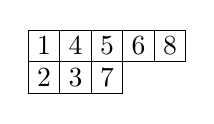
\begin{tikzpicture}[scale=0.4]\drawtbx{{1,4,5,6,8},{2,3,7}}{(0,0)}
\end{tikzpicture}.\end{center}
\end{example}

\begin{definition}\label{def:poly}
For a subgroup $G\leq \mathfrak{S}_n$, the \emph{signed sum of $G$} is an element in the group algebra given by the sum of $\sgn(\sigma)\sigma$ over all $\sigma\in G$.  

For an $(n-k,k)$-tableau, the \emph{polytabloid associated to $\tbx$} is the element $\{\tbx\}\kappa_{\tbx,\ell}\in \F\Omega_k$, where $\kappa_{\tbx}$ is the signed sum of $C_{\tbx}$.  We say that $\bfe_{\tbx}$ is \emph{standard} if so is $\tbx$.
\end{definition}

Note that a polytabloid is dependent on the defining tableau, i.e. row-equivalent but distinct tableaux can define distinct polytabloids.
For convenience, we will denote by $\bfe_{\omega}$ the polytbaloid $\bfe_{\tbx^{\omega}}$.

\begin{example}
For $n=8$, the polytabloid associated to $\tbx:= \tbx^{\interval{3}}$ is
\[
\bfe_{\interval{3}} = \{1,2,3\} - \{4,2,3\} - \{1,5,3\} +\{4,5,3\}.
\]
\end{example}

\medskip

%Suppose $\ell,k$ are non-negative integers with $\ell\leq k$ and $\ell\leq n-k$.
%Consider the element
%\[
%\bfe_{k,\ell} := \{1,2,\ldots,k\} \sum_{\sigma\in C_{k,\ell}} \sgn(\sigma)\sigma \;\;\in \F\Omega_k,
%\] 
%where $C_{k,\ell}$ is the direct product of $\langle (i,i+k)\rangle$ over all $i\in\interval{\ell}$.
%Note that $\bfe_{0,0}=0$.
\begin{definition}
For an integer $k$ with $n-2k\geq 0$, the \emph{Specht module} $S^{(n-k,k)}$ associated to a partition $(n-k,k)$ of $n$ is the $\F\mathfrak{S}_n$-submodule of $\F\Omega_k$ spanned by all polytabloids, i.e.
\[
S^{(n-k,k)} := \F\text{-span}\{ \bfe_{\tbx} \mid \tbx\text{ a $(n-k,k)$-tableau}\}.
\]
\end{definition}

Note that, if $\tbx'=\tbx \sigma$ for some $\sigma\in\mathfrak{S}_n$, then one can easily see that $\bfe_{\tbx'} = \bfe_{\tbx\sigma} = \bfe_{\tbx}\sigma$.
In particular, $S^{(n-k,k)}$ is generated (over $\F\mathfrak{S}_n$) by any single polytabloid.

From the viewpoint of representation theory over $\mathfrak{S}_n$, the map $\varphi_k$ was first studied by James (in the more general setting of any permtation module).  Namely, he uses it to produce a filtration of a permtation module with subquotient being Specht; see \cite{James3} for details.  We will only need the following results.

\begin{theorem}\label{thm:James}
Let $k$ be an integer with $2k\in\interval{0,n}$.  Then the following hold.
\begin{enumerate}
\item {\rm\cite{James1}} If $p\neq 2$, then $S^{(n-k,k)}$ has an irreducible top $D^{(n-k,k)}:=S^{(n-k,k)}/\mathrm{rad}S^{(n-k,k)}$.

\item {\rm\cite[Theorem 9.1]{James2}} $S^{(n-k,k)}\subset \Ker(\varphi_k)$.

\item {\rm \cite[Theorem 12.1]{James3}} The multiplicity of the simple module $D^{(n-k,k)}$ in the permutation module $M^{(n-k,k)}=\F\Omega_k$ is $1$.
\end{enumerate}
\end{theorem}

In \cite{Pe}, Peel considered a total order on the set of tabloids ($k$-subsets in our setting) and use it to show by induction that polytabloid associated to standard tableaux spans the Specht module.  In fact, this is one idea that leads to the above theorem in \cite{James2}, which in turn can be used to find a filtration for general permutation modules of the symmetric group; see \cite{James2, James3} for details.  Let us review this total order now.

\begin{definition}\label{def:Sa-order}
Denote by $\omega\ulhd_r\omega'$ if $|\omega\cap \interval{i}| \leq |\omega'\cap \interval{i}|$ for all $i\in\interval{k}$; this defines a partial order on $\Omega_k$ called the the \emph{row-dominance order}.
\end{definition}
\begin{remark}\label{rmk:orders}
The definition in \cite{James2} is stated differently. They use the backward-reading lexicographical order on $k$-subsets, i.e. $\omega <_{lex} \omega' \in \Omega_k$ if there is some $j\in \interval{k}$ so that $|\omega\cap\interval{j}|<|\omega'\cap\interval{j}|$ and $|\omega\cap\interval{i}|=|\omega'\cap \interval{i}$ for all $i\in\interval{j+1,k}$.
Our formulation is the opposite of the partial order used in \cite{Sag}, which is coarser than the one used in \cite{James2}.
With respect to the next result, it does not matter which order one prefer to use.
\end{remark}

\begin{theorem}\label{thm:Spechtbasis}
The following hold for any integer $k$ with $2k\in\interval{0,n}$.
\begin{enumerate}[(1)]
\item {\rm\cite[7.4]{James2}} Consider the poset $(\mathrm{Supp}(\bfe_{\tbx}), \ulhd_r)$ of supports of $\bfe_{\tbx}\in S^{(n-k,k)}$ under the row-dominance order.  If $\tbx$ is standard, then $\{\tbx\}$ is minimal in $\mathrm{Supp}(\bfe_{\tbx})$.

\item {\rm \cite{Pe},\cite[9.4]{James2}} The set $\{ \bfe_{\tbx}\mid \tbx\in \ST_n(k)\}$ of standard polytabloid forms a basis of $S^{k,\ell}$.
\end{enumerate}
\end{theorem}


% % % % % % % % % % % % % % % % % % % % % % % % % % % % % % 
% % % % % % % % % % % %  Basis Thm  % % % % % % % % % % % % 
% % % % % % % % % % % % % % % % % % % % % % % % % % % % % % 

\section{Basis of the slash homology groups}\label{sec:basis}

From now on, we impose the following
\[
\text{\bf Assumption}: \qquad n-2k \in \interval{0,p-2},
\]
unless otherwise stated.

\comm{TODO: rewrite this para}
Recall from Theorem \ref{thm:Spechtbasis} that the set $\ST_n(k)$ of standard Young $(n-k,k)$-tableaux is an indexing set of a basis (given by standard polytabloid) of $S^{k,k}$, and from Lemma \ref{lem:main-lo} that $H_k^{/0}$ is a quotient of $S^{k,k}$.
Moreover, there is also a well-known bijection between $\mathcal{L}_{n-k,k}^{1,\infty}$ with $\ST_n(k)$, so given that $\dim H_k^{/0}$ coincide with $|\mathcal{L}_{n-k,k}^{1,p-1}|$ as shown in the previous section, it is natural to expect the bijection induces a basis for $H_k^{/0}$.
The aim of this subsection is to show that this is indeed the case.

\begin{definition}\label{def:p-std}
We call a $(n-k,k)$-tableau $\tbx$ \emph{$p$-standard} if $n-2k\in\interval{0,p-2}$, $\tbx$ is standard and satisfies $\tbx_{2,j}<\tbx_{1,j+p-2}$ for all $j\in\{1, 2, \ldots, k\}$.  Denote by $\ST_n^p(k)$ the set of $p$-standard $(n-k,k)$-tableaux.
\end{definition}
\begin{remark}
As far as we know, the terminology `$p$-standard' was first used in \cite{Kl}.
\end{remark}

Our second main theorem is the following.

\begin{theorem}\label{thm:basis}
Suppose $k$ is an integer satisfying $n-2k\in\interval{0,p-2}$.
Then a basis of the slash homology group $H_k^{/0}$ is given by \[
\{[\bfe_\tbx] \mid \tbx \text{ is a $p$-standard tableau of shape $(n-k,k)$ } \},
\]
where $[v]$ denotes $v+\Image(\varphi_{k-p+1}^{p-1}) \in H_k^{/0}$ for $v\in \Ker(\varphi_k)$.
\end{theorem}

\begin{corollary}
For an integer $k$ satisfying $n-2k\in\interval{0,p-2}$, the simple top $D^{(n-k,k)}$ of $S^{(n-k,k)}$ admits a basis $\{[\bfe_\tbx] \mid \tbx \in \ST_n^p(k) \}$, where $[v]$ represents $v+\mathrm{rad} S^{(n-k,k)}$.
In particular, we have
\[
\dim_{\F} D^{(n-k,k)} = \sum_{j\in \Z} \binom{n}{pj+k} - \binom{n}{pj+k-1},
\]
where the binomial coefficient $\binom{a}{b}$ with $a$ or $b$ negative is considered zero.
\end{corollary}
\begin{remark}
The dimension formula is also obtained in \cite{Erd} (precisely, \cite[Example 5.3]{Erd} by taking $(m, s, t, d, \delta)$ therein as $(k, n-2k, 0, n-2k+1, p-(n-2k+1))$), which is proved by looking at tensor product of tilting modules over $GL_2(\F)$ and utilising Schur-Weyl duality.
\end{remark}
\begin{proof}
By Theorem \ref{thm:newfinal}, we have $D^{(n-k,k)}\cong H_k^{\slash 0}$.
Also, recall from Theorem \ref{thm:James} (3) that the appearance of $D^{(n-k,k)}$ in the composition factors of $M^{(n-k,k)}=\F\Omega_k$ is unique.  So the first part now follows immediately from Theorem \ref{thm:basis}.

For the dimension formula, we use the bijection between standard $(n-k,k)$-tableau and Dyck paths.  Recall that a Dyck path is a lattice path in $\Z^2$ starting at $(0,0)$ ending at $(n,n)$ that is (non-strictly) bounded by the $x$-axis and the diagonal $y=x$, and that each step of the path is either $(0,1)$ or $(1,0)$.  This bijection sends a standard tableau $\tbx$ to the path so that the $i$-th step is $(1,0)$ if $i$ is in the first row of $\tbx$; $(0,1)$ otherwise. c.f. \cite[p.4-5]{Moh}.

Under this bijection, the $p$-standard tableaux correspond to the Dyck paths that are (non-strictly )bounded in the region $0 \leq y-x < p$. Hence the dimension of $D^{(n-k,k)}$ for $n-2k\in\interval{0,p-2}$ is the same as the number of such Dyck paths.  The claim then follows by using existing formula for lattice path enumeration - for example, taking $(s,t)=(1,p-1)$ in \cite[Theorem 2]{Moh}.
\end{proof}


We will prove Theorem \ref{thm:basis} in what follows.
The strategy is to modify the \emph{straightening rule} - the induction process that is used to show that a Specht module admits a basis given by standard polytabloids in \cite{Pe}.  The modification are designed so that we can keep track of how ``far" away the tableaux appearing in a Garnir relation is from being a $p$-standard tableau.

\subsection{Preliminaries}\label{subsec:basisprelim}
In this subsection, we present the definition of the partially ordered set that allows us to prove Theorem \ref{thm:basis} by induction, and also a few techniques that we will use frequently.

For convenience, denote by
\[
\pbad_n(k) := \ST_n(k)\setminus \ST_n^p(k),
\]
and call its elements \emph{$p$-bad} standard tableaux.

\begin{definition}\label{def:aST}
Let $\tbx$ be a $(n-k,k)$-tableau.
\begin{enumerate}[(1)]
%\item Denote by $\tbx \lhd_c \tbx'$ if $\{\tbx\}^c=\{\tbx\}$

\item We say that $\tbx$ \emph{almost standard} if all of the following hold.
\begin{itemize}
\item $\tbx$ is column-standard (i.e. entries increase as we go down each column);
\item $\tbx$ is second-row-standard (i.e. entries in the second row increase as we go right).
\end{itemize}
Denote by $\aST:=\aST_n(k)$ the set of almost standard $(n-k,k)$-tableaux.

\item Define a partial order $\preceq$ on $\aST$ by declaring $\tbx\preceq\tbx'$ if one of the following conditions are satisfied.
\begin{enumerate}[(i)]
\item $\tbx=\tbx'$.
\item $|\{\tbx\}\cap\interval{i}|\leq |\{\tbx'\}\cap\interval{i}|$ for all $i\in\interval{n}$ with at least one of the inequalities being strict.
\item $\{\tbx\}=\{\tbx'\}$ and for the complement set $\interval{n}\setminus\{\tbx\} =\{x_1 < x_2 < \cdots < x_{n-k}\}$, there is some $j\in\interval{k}$ such that
\begin{itemize}
\item $x_i$ lies in the same position in both $\tbx,\tbx'$ for all $i<j$, and
\item $x_j=\tbx_{1,a}=\tbx_{1,b}'$ with $a>b$.
\end{itemize}
\end{enumerate}
This defines a partial order on $\aST$. 
%\comm{NOTE TO SELF: good/standard tableaux is 'largest' in $\aST$.}
\end{enumerate}
\end{definition}
The second condition on $\preceq$ is just the row-dominance order of Definition \ref{def:Sa-order}; we view this as a measure on how far a standard tableau is from being $p$-standard.
The last condition is used to measure how far an almost standard tableau from being standard, it is the partial order used in the proof of standard polytabloid basis of Specht modules in \cite{Pe,James2}  ``restricted to the first row".

Note that the standard $(n-k,k)$-tableaux are totally ordered by the row-dominance order.  This implies that, by combining with condition (iii), $(\aST,\preceq)$ is a totally ordered set.

\begin{example}
For $(n,k)=(5,2)$, then $(\aST,\preceq)$ is as follows, where the standard ones are shown in the top row.
\begin{center}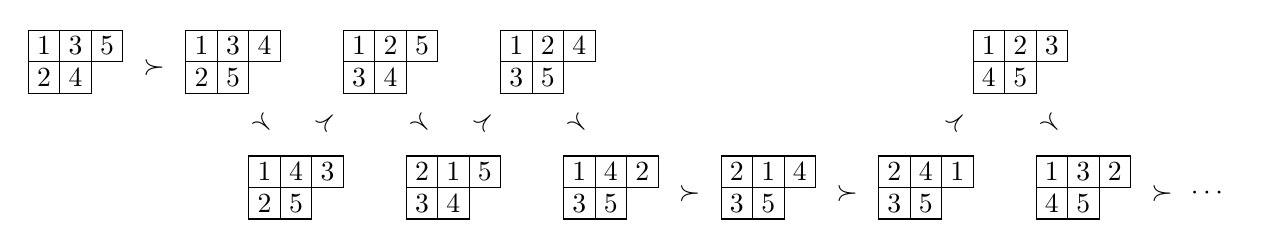
\begin{tikzpicture}[scale=0.4]
\node at (4.5,-0.7) {$\succ$};
\node[rotate=-45] at (8,-2.5) {$\succ$};
\node[rotate=45] at (10,-2.4) {$\succ$};
\node[rotate=-45] at (13,-2.5) {$\succ$};
\node[rotate=45] at (15,-2.4) {$\succ$};
\node[rotate=-45] at (18,-2.5) {$\succ$};
\node[rotate=45] at (30,-2.4) {$\succ$};
\node[rotate=-45] at (33,-2.5) {$\succ$};
\node at (21.5, -4.7) {$\succ$};
\node at (26.5, -4.7) {$\succ$};
\node at (36.5, -4.7) {$\succ$};
\node at (38,-4.7) {$\cdots$};

\drawtbx{{1,3,5},{2,4}}{(0,0)} 
\drawtbx{{1,3,4},{2,5}}{(5,0)} 
\drawtbx{{1,2,5},{3,4}}{(10,0)} 
\drawtbx{{1,2,4},{3,5}}{(15,0)} 
\drawtbx{{1,2,3},{4,5}}{(30,0)} 
\drawtbx{{1,4,3},{2,5}}{(7,-4)} 
\drawtbx{{2,1,5},{3,4}}{(12,-4)} 
\drawtbx{{1,4,2},{3,5}}{(17,-4)} 
\drawtbx{{2,1,4},{3,5}}{(22,-4)} 
\drawtbx{{2,4,1},{3,5}}{(27,-4)} 
\drawtbx{{1,3,2},{4,5}}{(32,-4)} 
\end{tikzpicture}\end{center}
Note that only the largest tableau $\tbx^{\{2,4\}}$ is good when $p=3$; for any prime $p>3$, all standard tableaux are good.
\end{example} 


Recall the following Garnir relation that is used to straighten a $(n-k,k)$-tableaux (with non-standard first row); c.f. \cite[Section 7, 8]{James3}.
\begin{lemma}\label{lem:Garnir}
Let $\tbx$ be a $(n-k,k)$-tableau.
%\begin{enumerate}[(1)]
%\item\label{itm:row1} 
For a positive integer $j\leq k$, the following equation holds.
\[
\bfe_\tbx = \bfe_\tbx\tau_{\tbx,j} - \bfe_\tbx \sigma_{\tbx,j},
\]
where $\tau_{\tbx,j}:=(\tbx_{1,j}, \tbx_{1,j+1})$ and $\sigma_{\tbx,j}:=(\tbx_{1,j}, \tbx_{1,j+1}, \tbx_{2,j})$.
\end{lemma}

\begin{lemma}\label{lem:col-swap}
The following hold for a $(n-k,k)$-tableau $\tbx$.
\begin{enumerate}[(1)]
\item Take $i<j\in\interval{k}$ and define the following \emph{column reordering} permutation. 
\[
\rho_{\tbx,i,j} := (\tbx_{1,j}, \tbx_{1,j-1}, \ldots, \tbx_{1,i+1})(\tbx_{2,j}, \tbx_{2,j-1}, \ldots, \tbx_{2,i+1})
\]
in $\mathfrak{S}_n$, then $\bfe_{\tbx}=\bfe_{\tbx}\rho_{\tbx,i,j}$.

\item If $(\tbx_{i,j})\sigma=\tbx_{i,j}$ for all $i\in\{1,2\}$ and $j\in\interval{k}$, then $\bfe_{\tbx}=\bfe_{\tbx}\sigma$
\end{enumerate}
\end{lemma}
\begin{proof}
Both of them follow immediately from the definition of polytabloid.
\end{proof}

\begin{lemma}\label{lem:bad-swap}
Consider almost standard tableaux $\tbx,\tbx'\in \aST$.
If $\{\tbx\}$ and $\{\tbx'\}$ differ only by one element, say $\{\tbx\}=S\sqcup\{a\}$ and $\{\tbx'\}=S\sqcup \{b\}$, and $a>b$, then $\tbx\prec \tbx'$.
\end{lemma}
\begin{proof}
Condition (ii) in Definition \ref{def:aST} holds by assumption.
\end{proof}
Colloquially, Lemma \ref{lem:bad-swap} says that if we replace an entry in the second row of an almost standard tableau by a smaller value, then the new almost standard tableau (after an appropriate column reordering if needed) is larger than the original one, in the $\preceq$-order.

\begin{lemma}\label{lem:nonstd}
If $\tbx\in \aST$ is a non-standard almost standard tableau, then $\bfe_{\tbx}\in \Fspan\{\bfe_{\tbx'}\mid \tbx'\succ \tbx\}$.
\end{lemma}
\begin{proof}
By non-standardness, we have an integer $j\in\interval{n-k}$ so that  $\tbx_{1,j}>\tbx_{1,j+1}$.
If $j\geq k$, then it follows from Lemma \ref{lem:col-swap} (2) that $\bfe_\tbx = \bfe_{\tbx}(\tbx_{1,j},\tbx_{1,j+1})$.
But $\tbx(\tbx_{1,j},\tbx_{1,j+1}) \succ \tbx$ by Definition \ref{def:aST} (2) (iii), so the claim follows.

Now we can assume $j\leq k$.
By Lemma \ref{lem:Garnir}, we have $\bfe_{\tbx} = \bfe_{\mathtt{u}}-\bfe_{\mathtt{v}}$, where $\mathtt{u}=\tbx\tau_{\tbx,j}$ and $\mathtt{v}=\tbx\sigma_{\tbx,j}$.
It is easy to see that $\mathtt{u}$ is almost standard and $\mathtt{u}\succ \tbx$.

Let $i$ be the unique integer so that $\tbx_{2,i} < \tbx_{1,j} < \tbx_{2,i+1}$.
Note that from the conditions we have $\tbx_{2,i}<\tbx_{1,j}<\tbx_{2,j}$, so $i<j$ as $\tbx$ has standard second-row.
By Lemma \ref{lem:col-swap}, we have $\bfe_{\mathtt{v}} = \bfe_{\mathtt{v}}\rho_{\mathtt{v},i,j}$.
Hence, we have $\bfe_{\tbx}=\bfe_{\mathtt{u}}-\bfe_{\mathtt{v}}\rho_{\mathtt{v},i,j}$, so it remains to show that $\mathtt{w}:=\mathtt{v}\rho_{\mathtt{v},i,j}\succ \tbx$.

By the choice of $\sigma_{\tbx,j}$, $\mathtt{v}$ is column-standard, and so the choice of $i,j$ now ensures that $\mathtt{w}\in \aST$.  Note also that swapping columns (by $\rho_{\mathtt{v},i,j}$) does not change the underlying set $\{\mathtt{v}\}$, i.e. $\{\mathtt{w}\}=\{\mathtt{v}\}$.
Since $\tbx_{2,j}>\tbx_{1,j}$ (by column-standardness of $\tbx$), $\{\mathtt{w}\}=\{\mathtt{v}\}$ is obtained from replacing $\tbx_{1,j}$ in $\{\tbx\}$ by the smaller $\tbx_{2,j}$.
So it follows from Lemma \ref{lem:bad-swap} that $\mathtt{w}\succ \tbx$ as required.%(1) The permutation $(\mathtt{s}_{1,i},\mathtt{s}_{1,j})(\mathtt{s}_{2,i},\mathtt{s}_{2,j})$ that swaps two columns of $\mathtt{s}$, and so it stabilises $\bfe_{\mathtt{s}}$, so the equation follows immediately from that of Lemma \ref{lem:Garnir}.
%(2) The definition of the permutations $\sigma_{\tbx,j}^{(r)}$ ensures that the new tableaux are always second-row-standard and column-standard.
%(3) Column-dominance follows from Lemma \ref{lem:cdom-dec}.
%As $\sigma_{\tbx,j}^{(2)}$ fixes all entries in the second row, the second part of the claim follows from the definition of the partial order $<_a$.
%(4) Let $\tbx':=\tbx\sigma_{\tbx,j}^{(3)}$ and $\omega:=\{\tbx'\}$.
%The permutation $\sigma_{\tbx,j}^{(3)}$ pushes the smaller entries $\tbx_{1,j},\tbx_{2,j}$ to a column on the left of the column containing $\tbx_{1,i},\tbx_{2,i}$, so by Lemma \ref{lem:cdom-dec} we have $\tbx\sigma_{\tbx,j}^{(3)}\lhd_c\tbx$.
%By construction, we have $\tbx_{2,i+\ell}>\tbx_{2,i+\ell}'$ for all $\ell>1$ and $\tbx_{2,i+\ell}=\tbx_{2,i+\ell}'$ for all $\ell\leq 0$.
%Thus, if $\tbx_{2,j} \geq 2j-1+p-1$, then by the choice of $\overline{\sigma}_{\tbx,j}^{(3)}$ we have $a(\tbx')<a(\tbx)$ (note that the two transposition acted on $\mathtt{s}$ has no effect on disparity); otherwise, we have $a(\tbx')=a(\tbx)$.
%(5) Immediate from (3) and (4).
\end{proof}

The motivation for the previous lemma should be natural: we want to do induction on $(\aST, \preceq)$.  In contrast, it may be unclear what the motivation of the forthcoming lemma is; we hope the reader can bear with us for the while as its use will be clear in the next subsection (specifically, Lemma \ref{lem:badstd}).

For a standard tableau $\tbx\in \ST_n(k)$, we define 
\[
\aST_\tbx:=\Bigl\{ \tbx' \in \aST \Bigm| \{\tbx'\}=\{\tbx\} \Bigr\} \subset \aST.
\]
In particular, $\tbx$ is the only standard tableau in $\aST_{\tbx}$ and is also the maximum in $(\aST_{\tbx}, \preceq)$.
\begin{lemma}\label{lem:nonstd2}
For any $\tbs\in \aST_\tbx$, we have 
\[
\bfe_{\tbs} \in \bfe_{\tbx}+\Fspan\{\bfe_{\tbx'}\mid  \tbx \prec \tbx'\in \aST \}.
\]
\end{lemma}

\begin{proof}
We prove this by induction (from large to small)  on $(\aST_\tbx, \preceq)$.
The claim is trivial for the case when $\tbs=\tbx$, which is the maximum of $(\aST_\tbx, \preceq)$.
Suppose $\tbs\neq \tbx$.
We can assume that $\tbs_{1,k+1} < \tbs_{1,k+2} < \cdots <\tbs_{1,n-k}$ by Lemma \ref{lem:col-swap} (2), which means that there exists $j\in\interval{k}$ so that $\tbs_{1,j}>\tbs_{1,j+1}$.

Following the same argument and notation as in the proof of Lemma \ref{lem:nonstd} yields $\bfe_{\tbs} = \bfe_{\mathtt{u}}-\bfe_{\mathtt{w}}$, where $\mathtt{u}:=\tbs\tau_{\tbs,j}$ and $\mathtt{w}:=\tbs\sigma_{\tbs,j}\rho$ with $\rho$ the column reordering permutation $\rho$ that ensures $\mathtt{w}$ is almost standard.

On one hand, the construction of $\mathtt{u}$ means that it is in $\aST_\tbx$ and also satisfies $\mathtt{u}\succ \tbs$, so it follows from induction hypothesis that
\[
\bfe_{\mathtt{u}} \in \bfe_{\tbx} + \Fspan\{\bfe_{\tbx'}\mid \tbx\prec\tbx'\in\aST\}.
\]
On the other hand, the same argument as in the proof of Lemma \ref{lem:nonstd} yields $\mathtt{w}\succ \tbs \succ \tbx$ (while $\mathtt{w}$ is not in $\aST_\tbx$).
Therefore, combining with $\bfe_{\tbs}=\bfe_{\mathtt{u}}-\bfe_{\mathtt{w}}$, the claim follows.
\end{proof}


\subsection{The case of bad tableaux}\label{subsec:badtab}
The aim of this subsection is to show a similar statement as Lemma \ref{lem:nonstd} but with $\tbx$ being a bad standard tableau and with the polytabloids replaced by their cosets in $H_k^{/0}$.

We start with the following key lemma which provides a relation between certain polytabloids in $H_k^{/0}$.
\begin{lemma}\label{lem:tbx-reln}
For a $(n-k,k)$-tableau $\tbx$ and an integer $i\in \interval{k-(p-2)}$, consider the $(p-1)$-subset $B:=\{\tbx_{1,i}, \tbx_{1,i+1}, \ldots, \tbx_{1,i+p-2}\}$, the following equation holds.
\[
\bfe_\tbx \sum_{\tau\in \mathfrak{S}_B} \tau = (\bfe_{\tbx'}\cdot K)\varphi^{p-1},
\]
where $\tbx'$ is the tableau obtained from $\tbx$ by removing all the columns containing an element of $B$, and $K$ is the set consisting of all the entries in these removed columns.
\end{lemma}
We remark that Figure \ref{fig:tbx} will be helpful to understand the statement.
\begin{proof}
Let us first set up some notations.
Take $\ell := |K \cap \{\tbx\}|\in\interval{0, p-2}$.
In particular, $\tbx'$ is a $(n-k-(p-1), k-\ell)$-tableau.
We take $L$ to be the set of entries in the first row that are not in $B$.  See Figure \ref{fig:tbx}.

\begin{figure}[!htbp]
\centering
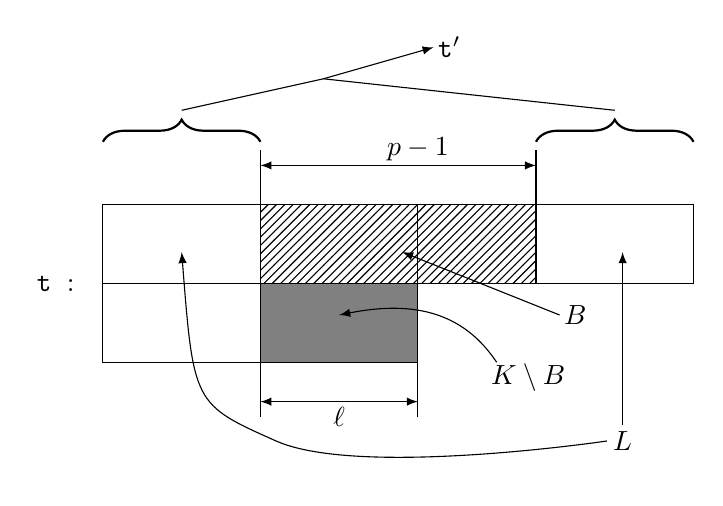
\begin{tikzpicture}
\node at (-0.6,1) {$\mathtt{t}$\;\;:};
\draw  (0,2) rectangle (4,0);
\draw  (0,2) rectangle (7.5,1);
\filldraw [pattern = north east lines]  (2,2) rectangle (5.5,1);
\filldraw [gray]  (2,1) rectangle (4,0);
\draw  (2,1) rectangle (4,0);

\draw[latex-latex] (2,2.5) -- (5.5,2.5);\draw (2,2) -- (2,2.7) (5.5,2)--(5.5,2.7);
\draw (4,2.7) node {$p-1$};

\draw[latex-latex] (2,-0.5) -- (4,-0.5);\draw (2,0) -- (2,-0.7) (4,0)--(4,-0.7);
\draw (3,-0.7) node {$\ell$};
\draw[decorate,decoration={brace,amplitude=0.8em},thick] (0,2.8) -- (2,2.8);
\draw[decorate,decoration={brace,amplitude=0.8em},thick] (5.5,2.8) -- (7.5,2.8);
\draw (1,3.2) -- (2.8,3.6) -- (6.5,3.2); \draw[-latex] (2.8,3.6)--(4.2,4);
\node at (4.4,4) {$\mathtt{t}'$};
\draw[latex-] (3,0.6) .. controls (4,0.8) and (4.6,0.6) .. (5,0); \node at (5.4,-0.2) {$K\setminus B$};
\draw[latex-]  (3.8,1.4) -- (5.8,0.6); \node at (6,0.6) {$B$};

\draw[latex-]  plot[smooth, tension=.7] coordinates {(1,1.4) (2.2,-1)  (6.4,-1)};
\draw[latex-] (6.6,1.4) -- (6.6,-0.8);
\node at (6.6,-1) {$L$};
\end{tikzpicture}
\caption{Notations used in Lemma \ref{lem:tbx-reln}.}\label{fig:tbx}
\end{figure}

We will prove the lemma by showing the following two equalities:
\begin{enumerate}[(i)]
\item $\bfe_\tbx \sum_{\tau\in \mathfrak{S}_B} \tau = -\bfe_{\tbx'}\cdot(K)\varphi^{(p-1)}$.
\item $-\bfe_{\tbx'}\cdot(K)\varphi^{(p-1)} = (\bfe_{\tbx'}\cdot K)\varphi^{p-1}$.
\end{enumerate}

\underline{Proof of (i)}: 
For clarity, what we need to show is the equality
\begin{equation}\label{eq:countB}
\sum_{\tau\in \mathfrak{S}_B} \sum_{\sigma\in C_{\tbx}} \sgn(\sigma)\{\tbx\}\sigma\tau = \sum_{\sigma' \in C_{\tbx'}} \sgn(\sigma')\big(\{\tbx'\}\sigma'\big) \cdot (K)\varphi^{(p-1)}.
\end{equation}

Consider a $k$-subset $\omega$ that is of the form $\{\tbx\}\sigma\tau$ with $\sigma\in \mathfrak{S}_B$ and $\tau\in C_\tbx$.
Let $\sigma'\in C_{\tbx'}$ be the unique element given by the restriction of $\sigma$ on $\tbx'$.
Then we can write $\omega = (\{\tbx'\}\sigma')\cdot (K\cap \omega)$.
Using Figure \ref{fig:tbx}, one can observe the following.
Firstly, the $\ell$-subset $K\cap\omega$, must  appear as a unique support of $(K)\varphi_{\ell+p-1}^{(p-1)}$.
Hence, $\omega$ must arise in the support in the right-hand side of \eqref{eq:countB}.
Secondly, for every $k$-subset in the said support, one can always obtain it in the form of $\{\tbx\}\sigma\tau$.

Now we need to show that the coefficients $\lambda_\omega$ and $\mu_\omega$ of $\omega$ in the left-hand side and right-hand side of \eqref{eq:countB}, respectively, coincide.

The number of times that $\omega$ is picked up in the summation over $\mathfrak{S}_B$ is the order of the stabiliser subgroup of $\omega$ in $B$.
Since this group is just $\mathfrak{S}_{(\interval{n}\setminus\omega)\cap B} \times \mathfrak{S}_{\omega\cap B}$, the number we need is $(p-1-r)!r!$, where $r=|\omega\cap B|$.
It follows from Wilson's theorem that $(p-1-r)!r!\equiv (-1)^{r+1}$ (mod $p$), so we have $\lambda_\omega = (-1)^{r+1}\sgn(\sigma)$, for $\omega = \{\tbx\}\sigma\tau$ as in \eqref{eq:countB}.
Now $\sgn(\sigma)$ is determined by the number of elements in $\omega$ that are not in $\{\tbx\}$.
This number is given by $|\omega\cap B| + |\omega \cap L|$, where $L=\{\tbx_{1,j}\mid j\in\interval{n-k}\setminus\interval{i,i+p-2} \}$.
Thus, the coefficient $\lambda_\omega$ is $(-1)^{2r+1+r'} = (-1)^{r'+1}$, where $r':=|\omega \cap L|$.

On the other hand, since the coefficient of every $k$-subset in the support of $(\kappa)\varphi^{(p-1)}$ is $1$, combining with $\omega = \{\tbx'\}\sigma'\cdot (K\cap\omega)$, we have $\mu_\omega = -\sgn(\sigma')$.
It then follows from the decomposition 
\[
\{\tbx'\}\sigma' = (\{\tbx\}\cap \omega) \sqcup (L\cap \omega)
\]
that $-\sgn(\sigma')=(-1)^{r'+1} = \lambda_\mu$.
This finishes the proof of (i).

\underline{Proof of (ii)}:
It is clear from the construction that every $k$-subset in the support of $\bfe_{\tbx'}$ is disjoint from $K$, so it follows from the splitting rule (Lemma \ref{lem:splitting}) that 
\[
(\bfe_{\tbx'}\cdot K)\varphi^{(p-1)} = \sum_{i=0}^{p-1} (\bfe_{\tbx'})\varphi^{(i)}\cdot (K)\varphi^{(p-1-i)}.
\]
It then follows from Theorem \ref{thm:James} that $\bfe_{\tbx'}\in S^{k-\ell,k-\ell}$ is annihilated by $\varphi^i = i! \varphi^{(i)}$ for any $i>0$, so we have $(\bfe_{\tbx'}\cdot K)\varphi^{(p-1)} = \bfe_{\tbx'}\cdot(K)\varphi^{(p-1)}$.  This finishes the proof of (ii).

The required equality now follows from the observation that $\varphi^{(p-1)}=(p-1)!\varphi^{p-1}=-\varphi^{p-1}$, where the last equality follows from Wilson's theorem.
\end{proof}

Before proceeding to the next step, we need an elementary observation on the elements in $\{\tbx^P\}$ that correspond to a $(0,1)$-step intersecting or lying below the line $y=x-(p-1)$.
\begin{lemma}\label{lem:badpaths}
Let $\tbx:=\tbx^P$ be a standard tableau associated to a path $P$, and $(x,y)$ be the starting point of the $i$-th (0,1)-step of $P$.
Then $(x,y)$ satisfies $y\leq x-(p-1)$ if, and only if, we have a strictly descending chain
\[\tbx_{2,i} > \tbx_{1,i+p-2} > \tbx_{1,i+p-3} > \cdots > \tbx_{1,i}.\]
In particular, $P$ is bad if, and only if, there is some $i\in \interval{k}$ such that $\tbx_{2,i}\geq 2i-1+p-1$; in which case, we also have $i+p-2\leq n-k$.
\end{lemma}
\begin{proof}
The if statement follows from $\tbx$ being standard and the correspondence between standard $(n-k,k)$-tableau and $\mathcal{L}_{n-k,k}^{1,\infty}$. 

For the only if part, by definition we have $y=i-1$, and so we have $x\geq i+p-2$.
Since $x$ counts the number of entries in the first row of $\tbx$ that are less than $\tbx_{2,i}$, so $x\geq i+p-2$ implies that $\tbx_{2,i}>\tbx_{1,i+p-2}$; the rest of the chain follows from the row-standardness of $\tbx$.

For the final statement, observe from the condition on the chain that the smallest possible value $\tbx_{2,i}$ can take is $(i+p-2)+(i-1)+1 = 2i-1+p-1$, where $i+p-2$ is the number of terms in the chain above that appear after $\tbx_{2,i}$ (hence the inequality $i+p-2\leq n-k$), and $(i-1)$ is the number of $\tbx_{2,j}$ satisfying $\tbx_{2,j}<\tbx_{2,i}$.
\end{proof}

Lemma \ref{lem:badpaths} allows us to introduce the following terminology.
\begin{definition}\label{def:Bi}
For a bad standard tableau $\tbx$, we say that $\tbx_{2,i}$ is a \emph{bad entry} if $\tbx_{2,i}\geq 2i-1+p-1$.
Since such an entry always exists by Lemma \ref{lem:badpaths}, we can  define the following $(p-1)$-subset of $\interval{n}$:
\[
B_i:=\{\tbx_{1,i+1} < \tbx_{1,i+2} < \cdots < \tbx_{1,i+p-1} < \tbx_{2,i}\}.
\]
\end{definition}

\begin{lemma}\label{lem:tbx-out}
Let $\tbx$ be a bad standard tableau with a bad entry $\tbx_{2,i}$.
Then the element $\sum_{\tau\in \mathfrak{S}_{B_i}} \bfe_{\tbx}\tau \in S^{k,k}$ belongs to the submodule $\Image(\varphi_{k+p-1}^{p-1})$.
\end{lemma}
\begin{proof}
Take $B:=B_i(\tbx_{1,i},\tbx_{2,i})$, then we have $(\tbx_{1,i},\tbx_{2,i})\mathfrak{S}_{B_i}(\tbx_{1,i},\tbx_{2,i}) = \mathfrak{S}_B$.
This implies that
\begin{align*}
\sum_{\tau\in\mathfrak{S}_{B_i}}\bfe_{\tbx}\tau  &=  \left(\sum_{\sigma \in \mathfrak{S}_B} \bfe_{\tbx}(\tbx_{1,i},\tbx_{2,i})\sigma\right) (\tbx_{1,i},\tbx_{2,i}) = -\left(\sum_{\sigma \in \mathfrak{S}_B} \bfe_{\tbx}\sigma\right) (\tbx_{1,i},\tbx_{2,i}),
\end{align*}
where the last equality follows from the observation that $\bfe_\tbx = -\bfe_\tbx(\tbx_{1,i},\tbx_{2,i})$.
On the other hand, it follows from Lemma \ref{lem:tbx-reln} that $\sum_{\sigma\in\mathfrak{S}_B}\bfe_{\tbx}\sigma \in \Image(\varphi^{p-1})$.
Hence, the element on the right-hand side is also in $\Image(\varphi^{p-1})$, and so is $\sum_{\tau\in \mathfrak{S}_{B_i}} \bfe_\tbx \tau$.
\end{proof}


\begin{lemma}\label{lem:badpaths2}
Let $\tbx$ be a bad standard tableau with a bad entry $\tbx_{2,i}$.
Then $\tbx\sigma$ is column-standard for any $\sigma\in B_i$.
In particular, $\tbx\sigma$ is almost standard if $(\tbx_{2,i})\sigma=\tbx_{2,i}$.
\end{lemma}
\begin{proof} 
Column-standardness follows from the existence of the chain in Lemma \ref{lem:badpaths}.
More precisely, for $j \in \interval{p-2}$ with $i+j\leq k$, we have $(\tbx\sigma)_{2,i+j}=\tbx_{2,i+j}>\tbx_{2,i}\geq \tbx_{1,j+l}$ for all $l\in\interval{p-2}$ and so $\tbx_{2,i+j}>(\tbx\sigma)_{1,i+j}$ always.
For the $i$-th column, again the chain in Lemma \ref{lem:badpaths} tells us that $(\tbx_{2,i})\sigma\geq\tbx_{1,i+1}>\tbx_{1,i}=(\tbx\sigma)_{1,i}$.
The last statement follows from the fact that $\tbx$ is standard and $\sigma$ fixes all entries in the second row.
\end{proof}

Before proceeding, recall our notation 
\[\ [v]:=v+\Image(\varphi^{p-1}) \in H_k^{/0}\]
for the coset containing $v\in \F\Omega_k$ in the quotient $H_k^{/0}$.

\begin{lemma}\label{lem:badstd}
Suppose $\tbx$ is a bad standard tableau, then we have $[\bfe_{\tbx}] \in \Fspan\{[\bfe_{\tbx'}]\mid \tbx'\succ\tbx\}\subset H_k^{/0}$.
\end{lemma}
\begin{proof}
By Lemma \ref{lem:tbx-out}, if $\tbx_{2,i}$ is a bad entry (which always exists by Lemma \ref{lem:badpaths}), we have 
\[
-[\bfe_\tbx]=\sum_{1\neq \sigma\in \mathfrak{S}_{B_i}} [\bfe_{\tbx}\sigma]
\]
in $H_k^{/0}$.
So it suffices to show that $[\bfe_\tbx\sigma]$ with non-identity $\sigma\in \mathfrak{S}_{B_i}$ is in $\Fspan\{\bfe_{\tbx'}\mid \tbx'\succ\tbx\}$.

We partition $\mathfrak{S}_{B_i}\setminus\{1\}$ into two disjoint subsets $S\sqcup T$ so that $S$ consists of all the non-identity permutations $\sigma$ that fix $\tbx_{2,i}$.

By Lemma \ref{lem:nonstd2}, for any $\sigma\in S$, we have
\[
\bfe_{\tbx}\sigma \in \bfe_{\tbx} + \Fspan\{ \tbx' \in \aST \mid \tbx'\succ \tbx \}.
\]
Therefore, we have $\sum_{\sigma\in S} \bfe_\tbx \sigma = |S|\bfe_\tbx + v$ for some $v\in \Fspan\{\bfe_{\tbx'}\mid \tbx'\succ\tbx\}$.
Note that the subgroup $\{1\}\sqcup S$ of $\mathfrak{S}_{B_i}$ that stabilises $\tbx_{2,i}$ is of order $(p-2)!$, which is congruent to $1$ mod $p$ by Wilson's theorem.
This means that $|S|$ is congruent to $0$ mod $p$, which yields
\[
-[\bfe_\tbx] = (|S|[\bfe_\tbx]+[v])+\sum_{\sigma \in T}[\bfe_{\tbx}\sigma] =  [v]+\sum_{\sigma \in T}[\bfe_{\tbx}\sigma]
\]
with $v\in \Fspan\{\tbx'\mid \tbx'\succ\tbx\}$.

Now consider $\sigma\in T\subset \mathfrak{S}_{B_i}$.  
It follows from Lemma \ref{lem:badpaths2} that $\tbx\sigma$ is column-standard.
By Lemma \ref{lem:col-swap}, we can apply a column reordering permutation $\rho$ so that $\tbx\sigma\rho$ is almost standard and $\bfe_\tbx\sigma=\bfe_\tbx\sigma\rho$.
Since
\[
\{\tbx \sigma\rho\}=\{\tbx\sigma\} = \big(\{\tbx\}\setminus\{\tbx_{2,i}\}\big)\sqcup\{(\tbx_{2,i})\sigma\},
\]
and Lemma \ref{lem:badpaths} says that $(\tbx_{2,i})\sigma< \tbx_{2,i}$, applying Lemma \ref{lem:bad-swap} yields $\tbx\sigma\rho\succ \tbx$.

Thus, the summation $\sum_{\sigma\in T}[\bfe_\tbx\sigma]$ is in $\Fspan\{\tbx'\mid \tbx'\succ\tbx\}$, and the proof is now completed.
\end{proof}

All the required ingredients for proving Theorem \ref{thm:basis} are now ready.

\subsection{Proof of Theorem \ref{thm:basis}}\label{subsec:basisproof}
We can assume $\mathcal{L}_{n-k,k}^{1,p-1}$ is non-empty (in particular, $p\neq 2$); otherwise, there is nothing to show as $H_k^{/0}=0$.

By Lemma \ref{lem:main-lo}, $H_k^{/0}$ is a quotient of the Specht module $S^{k,k} = \Fspan\{\bfe_\tbx\mid \tbx:$ any tableau$\}$, which has a basis given by standard polytabloid.  So we can prove the theorem by showing the following result.

\begin{lemma}
For all $\tbx\in \aST$, we have
\[
\ [\bfe_{\tbx}] \in  \Fspan\{[\bfe_{\tbx'}]\mid \tbx'\text{ good and standard }\}.
\]
\end{lemma}
\begin{proof}
We will show this by induction on $(\aST,\preceq)$.
Note that the maximal (in fact, maximum) element of this poset is the standard tableau $\tbx^\omega$ associated to $\omega=\{2, 4, \ldots,2k\}$, which corresponds to the lattice path that changes direction at every step.
This path is in $\mathcal{L}_{n-k,k}^{1,p-1}$ so long as the set is non-empty.
Hence, there is nothing to show in the case $\tbx=\tbx^\omega$.

Consider now $\tbx\prec\tbx^\omega$.
If $\tbx$ is a good standard tableau, then there is nothing to show; otherwise, there are two possible form of $\tbx$ - a bad standard tableau or a non-standard tableau.

If $\tbx$ is a bad standard tableau, then it follows from Lemma \ref{lem:badstd} that $[\bfe_\tbx]\in \Fspan\{[\bfe_{\tbx'}] \mid \tbx'\succ \tbx\}$.

If $\tbx$ is non-standard, then 
we can assume that $\tbx_{1,k+1}< \tbx_{1,k+2}<\cdots <\tbx_{1,n-k}$ by Lemma \ref{lem:col-swap} (2).
Now, if $j$ is an integer with $\tbx_{1,j}>\tbx_{1,j+1}$, then $j\in\interval{k}$, and so it follows from Lemma \ref{lem:nonstd} that $[\bfe_\tbx]\in \Fspan\{[\bfe_{\tbx'}]\mid \tbx'\succ\tbx\}$.

Now we have shown that $[\bfe_\tbx]\in \Fspan\{[\bfe_{\tbx'}]\mid \tbx'\succ\tbx\}$ in the two possible forms of $\tbx$.
By induction hypothesis, for every $\tbx'\succ\tbx$ we have $[\bfe_{\tbx'}]\in \Fspan\{[\bfe_{\tbx''}]\mid \tbx''$ good and standard $\}$, hence it follows immediately that so is $[\bfe_\tbx]$.
\end{proof}

This completes the proof of Theorem \ref{thm:basis}.


\begin{thebibliography}{99999}
%\bibitem[BM]{BM} C.~Brennan; S.~Mavhungu.  Visits to level $r$ by Dyck paths.  {\it Fundamenta Informaticae} {\bf 117}, 2012, 127--145.
\bibitem[BJS]{BJS} S.~Bell; P.~Jones; J.~Siemons.
On modular homology in the {B}oolean algebra. {II}.
{\it J. Algebra} {\bf 199} (2), 1998, 556--580.

\bibitem[Erd]{Erd} K.~Erdmann.
Tensor products and dimensions of simple modules for symmetric groups. {\it Manuscripta Math.} {\bf 88}, 1995, 357--386.

\bibitem[J1]{James1} G.~D.~James.
The irreducible representations of the symmetric groups.  {\it Bull. London Math. Soc.} {\bf 8} (3), 1976, 229--232.

\bibitem[J2]{James2} G.~D.~James.
A characteristic-free approach to the representation theory of $\mathfrak{S}_n$.  {\it J. Algebra} {\bf 46} (2), 1977, 430--450.

\bibitem[J3]{James3} G.~D.~James.  The representation theory of the symmetric groups, Lecture Notes in Mathematics, vol. 682, Springer, Berlin, 1978.

\bibitem[Kap]{Kapranov} M.~M.~Kapranov. On the q-analog of homological algebra. preprint, arXiv:q-alg/9611005

\bibitem[KQ]{KhQi} M.~Khovanov; Y.~Qi.  An approach to categorification of some small quantum groups.  {\it Quantum Topol.} {\bf 6} (2), 2015, 185--311.

\bibitem[Kl]{Kl} A.~Kleshchev.  Completely splittable representations of symmetric groups.  {\it J. Algebra} {\bf 181} (2), 1996, 584--592.

\bibitem[M1]{Mayer1} W.~Mayer. A new homology theory I. {\it Ann. Math.} {\bf 43}, 1942, 370–380.

\bibitem[M2]{Mayer2} W.~Mayer. A new homology theory II. {\it Ann. Math.} {\bf 43}, 1942, 594–605.

\bibitem[Moh]{Moh} S.~G.~Mohanty. {\it Lattice path counting and applications.} Academic Press, New York-London-Toronto, Ont., 1979. xi+185 pp. ISBN: 0-12-504050-4

\bibitem[Pe]{Pe} M.~H.~Peel. Specht modules and the symmetric groups. {\it J. Algebra} {\bf 36}, 1975, 88-97.

\bibitem[Qi]{Qi} Y.~Qi.  Hopfological algebra.  {\it Compositio Mathematica} {\bf 150} (01): 1–45, 2014.

\bibitem[Sag]{Sag} B.~E.~Sagan. {\it The Symmetric Group: Representations, Combinatorial Algorithms, and Symmetric Functions.} Graduate Texts in Mathematics 203, Springer-Verlag, New York, 2001. xvi+240 pp. ISBN: 978-1-4419-2869-6

\bibitem[Wil]{Wil} M.~Wildon. The multistep homology of the simplex and representations of symmetric groups.  arXiv:1803.00465.
\end{thebibliography}
\end{document}